\pagenumbering{arabic}
%\documentclass[slides]{beamer}
\documentclass[mathserif, 10pt]{beamer}
\usepackage[framesassubsections]{beamerprosper}
\setbeamercovered{transparent}
%\documentclass[slides,hyperref={pdfpagelabels=false}]{beamer}
%\documentclass[handout,gray]{beamer}
\usepackage[T1]{fontenc}
\usepackage[utf8]{inputenc}
\usepackage{textcomp}
\usepackage{algorithm}
\usepackage{algorithmic}
\usepackage{color}
\usepackage{verbatim}
\usepackage{amsbsy}
\usepackage{multirow}
\usepackage{multicol}
\usepackage{booktabs} % Make some nice tables
\usepackage{ae,aecompl}

%%%%%%%%%%%% COULEURS %%%%%%%%%%%%%%%%%%%%%%%%%%%

\mode<presentation>
{
  \definecolor{beamerstructure}{RGB}{43,79,112}
  \definecolor{sidebackground}{RGB}{230,242,250}
  \definecolor{CTCC}{RGB}{133,188,228}
  \color{beamerstructure}
  \usetheme{default}
  \usepackage{courier}
  \beamertemplateballitem
\setbeamertemplate{navigation symbols}{}
%\setbeamertemplate{sidebar left}{\thispdfpagelabel{\insertframenumber}}
%\setbeamertemplate{footline}{\quad\insertframenumber}
%\usecolortheme{CTCC}
}
\usebackgroundtemplate{
\includegraphics[width=1.02\paperwidth]{../templets/ctcc_general.jpg}}

\title{\\\vspace{1cm}
Density Functional Theory with multiwavelets
}
%\subtitle{\textcolor{magenta}{My subtitle (if applicable)}}
\author{Stig Rune Jensen}
\institute[CTCC]{\\[-6mm]stig.r.jensen@uit.no\\[6mm]UiT - The Arctic University of Norway\\[6mm]

\includegraphics[height=1.5cm]{../templets/uio.pdf}\hspace{1cm} 

\includegraphics[height=1.5cm]{../templets/sff.pdf}\hspace{1cm}

\includegraphics[height=1.5cm]{../templets/uit.pdf}}
\date{Stony Brook, 4 August 2016}

\newcommand{\gb}[1]{green!#1!black}
\newcommand{\rb}[1]{red!#1!black}
\newcommand{\bb}[1]{blue!#1!black}
\newcommand{\coleq}{red!60!black}
\newcommand{\du}{\textrm{d}}
\newcommand{\ud}{\ensuremath{\,\mathrm{d}}}
\newcommand{\mymin}[1]{\underset{\hbox{\ensuremath{#1}}}{\text{min}}}

\newcommand{\red}[1]{\textcolor{red}{#1}}

\begin{document}

\footnotesize
\setlength{\unitlength}{\textwidth}

{
\usebackgroundtemplate{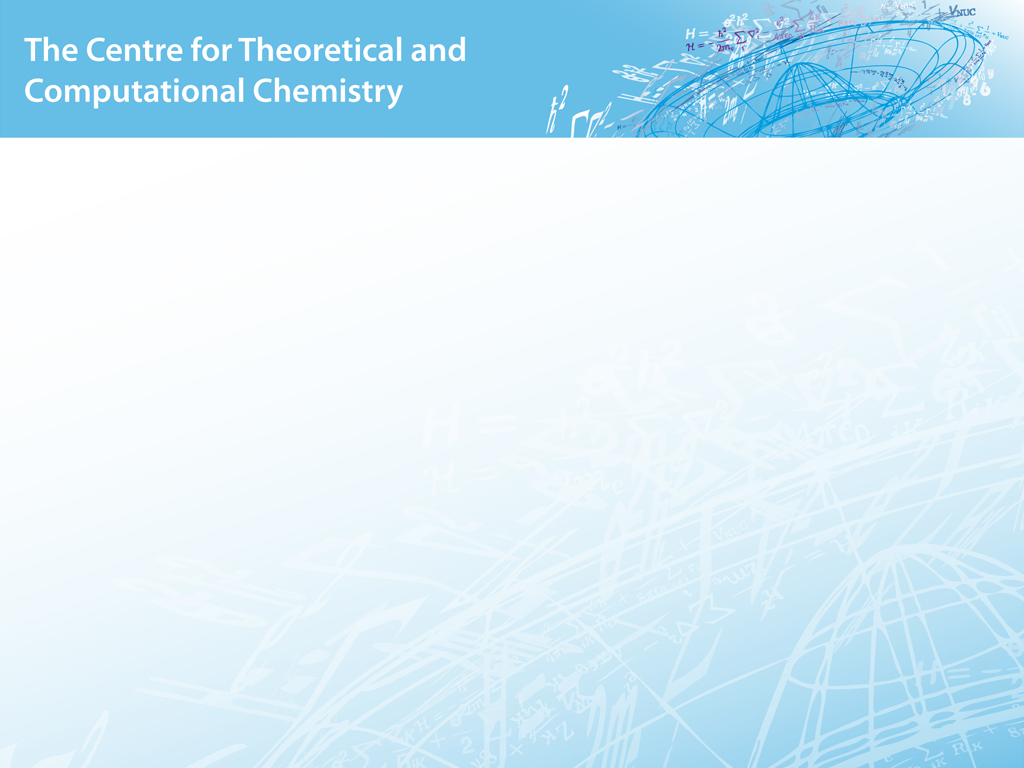
\includegraphics[width=1.02\paperwidth]{../templets/ctcc_forside.jpg}}
\maketitle
}

\begin{frame}
    \frametitle{Outlook}
    \begin{itemize}
	\item   \textbf{Density Functional Theory}
	\begin{itemize}
	    \item General DFT
            \item Hohenberg-Kohn
            \item Kohn-Sham
            \item XC energy and potential
            \item Kohn-Sham equations
            \item Total energy
	    \item Integral reformulation
	\end{itemize}
	\ \\
	\ \\
	\item   \textbf{Iterative algorithms}
	\begin{itemize}
            \item One-electron system
            \item Hydrogen atom
            \item Energy update
            \item KAIN
            \item Many-electron systems
            \item Fock/KS operator
            \item Orthonormalizations
            \item Fock matrix without kinetic operator
            \item Total energy without kinetic operator
            \item Orbital localization
            \item Lambda update
            \item Quadratic energy
            \item Final algorithm
	\end{itemize}
    \end{itemize}
\end{frame}

\begin{frame}
    \frametitle{The molecular Schr\"{o}dinger equation}
    \ \\
    \begin{equation}
	\nonumber
	\hat{H}\psi = E\psi
    \end{equation}
    \ \\
    \begin{equation}
	\nonumber
	\hat{H} =   -\sum_I \frac{\nabla^2}{2M_I} - \sum_i \frac{\nabla^2}{2}
		    +\sum_{I>J} \frac{Z_IZ_J}{|\boldsymbol{R}_I-\boldsymbol{R}_J|} 
		    -\sum_{i,I} \frac{Z_I}{|\boldsymbol{r}_i-\boldsymbol{R}_I|} 
		    +\sum_{i>j} \frac{1}{|\boldsymbol{r}_i-\boldsymbol{r}_j|} 
    \end{equation}
    \ \\
    \ \\
    \ \\
    \centering
    For an $N$-particle problem, the wave function is $3N$-dimensional
    \begin{equation}
	\nonumber
	\psi = \psi(\boldsymbol{r}_1,\boldsymbol{r}_2,\dots,\boldsymbol{r}_N)
    \end{equation}
    \ \\
    \ \\
    \ \\
    \pause
    \centering
    $\beta$-Carotene ($C_{40}H_{56}$) has 296 electrons and an 888-dimensional
    electronic wavefunction!
    \only<1>{
    \begin{center}
    %white background
    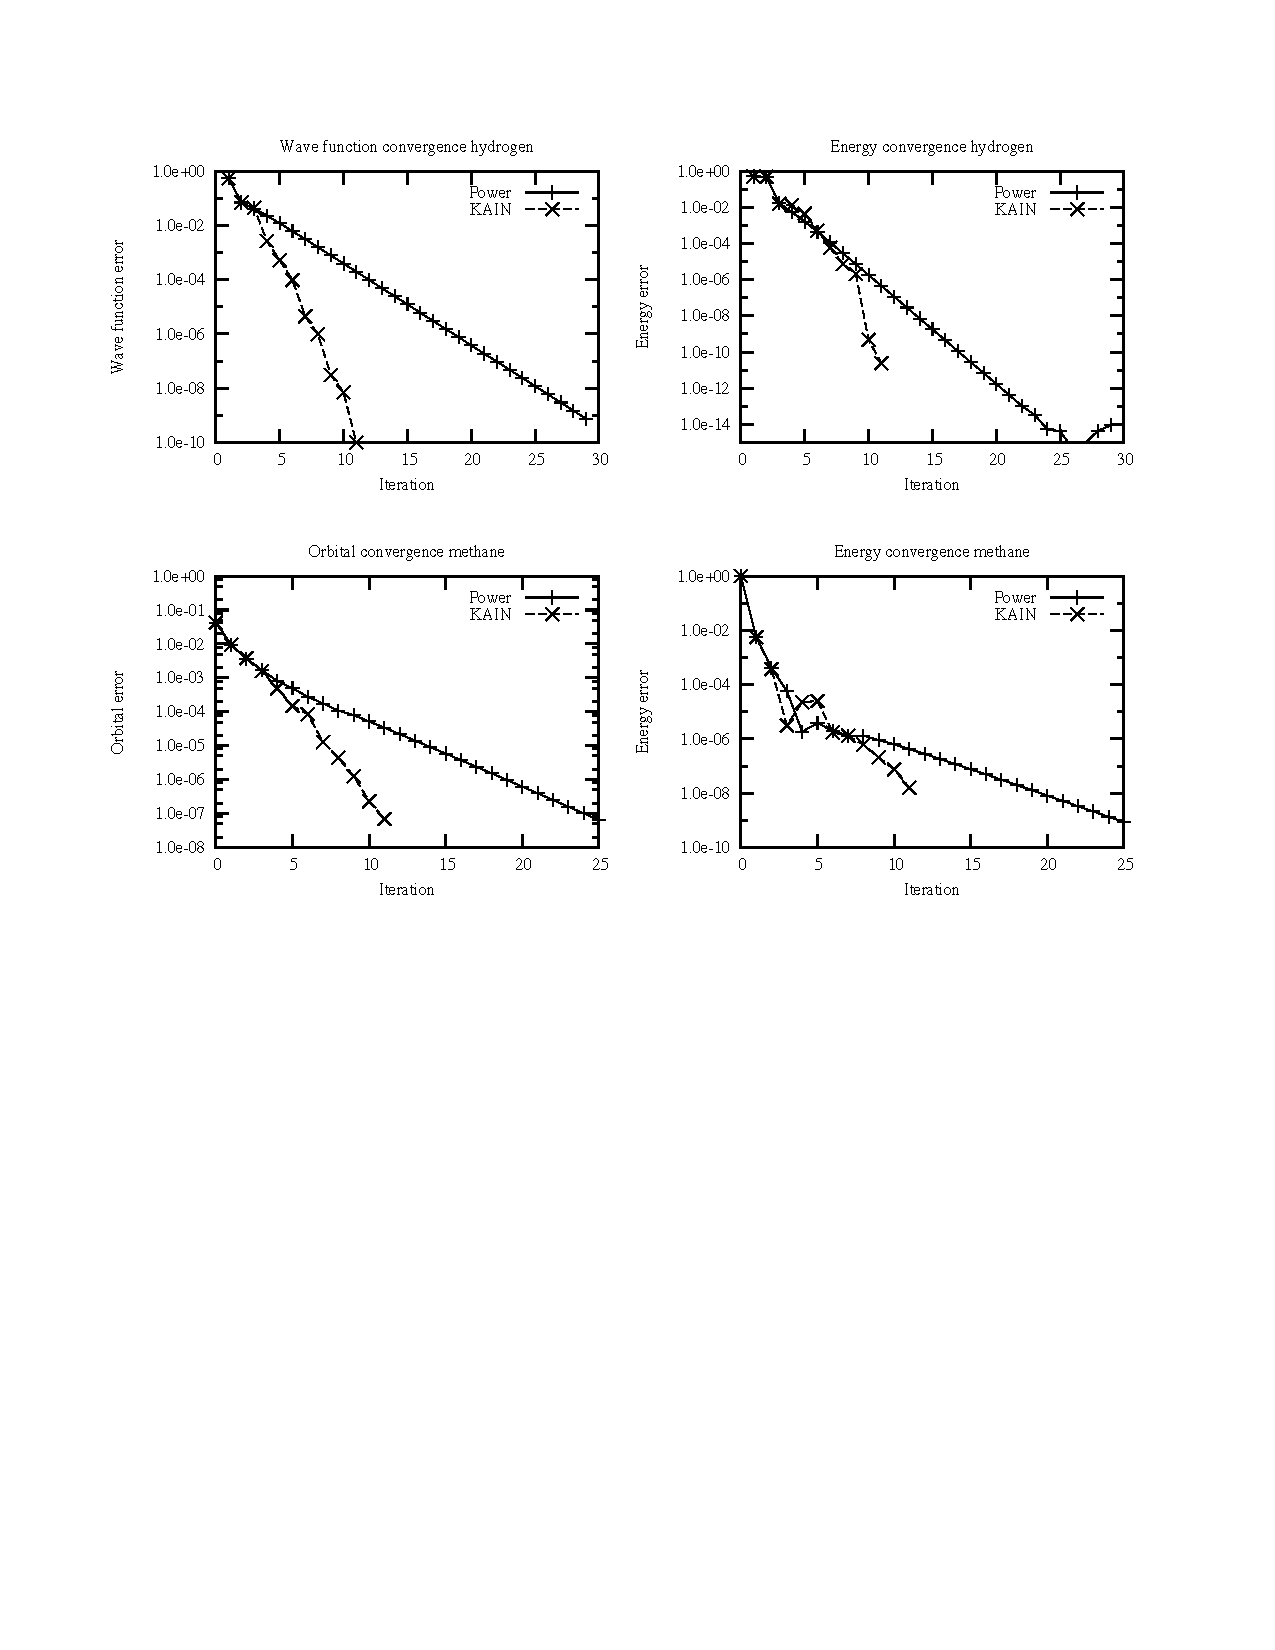
\includegraphics[scale=0.3, clip, viewport = 0 0 900 280]{figures/convergence.pdf}
    \end{center}
    }
    \only<2>{
    \begin{center}
    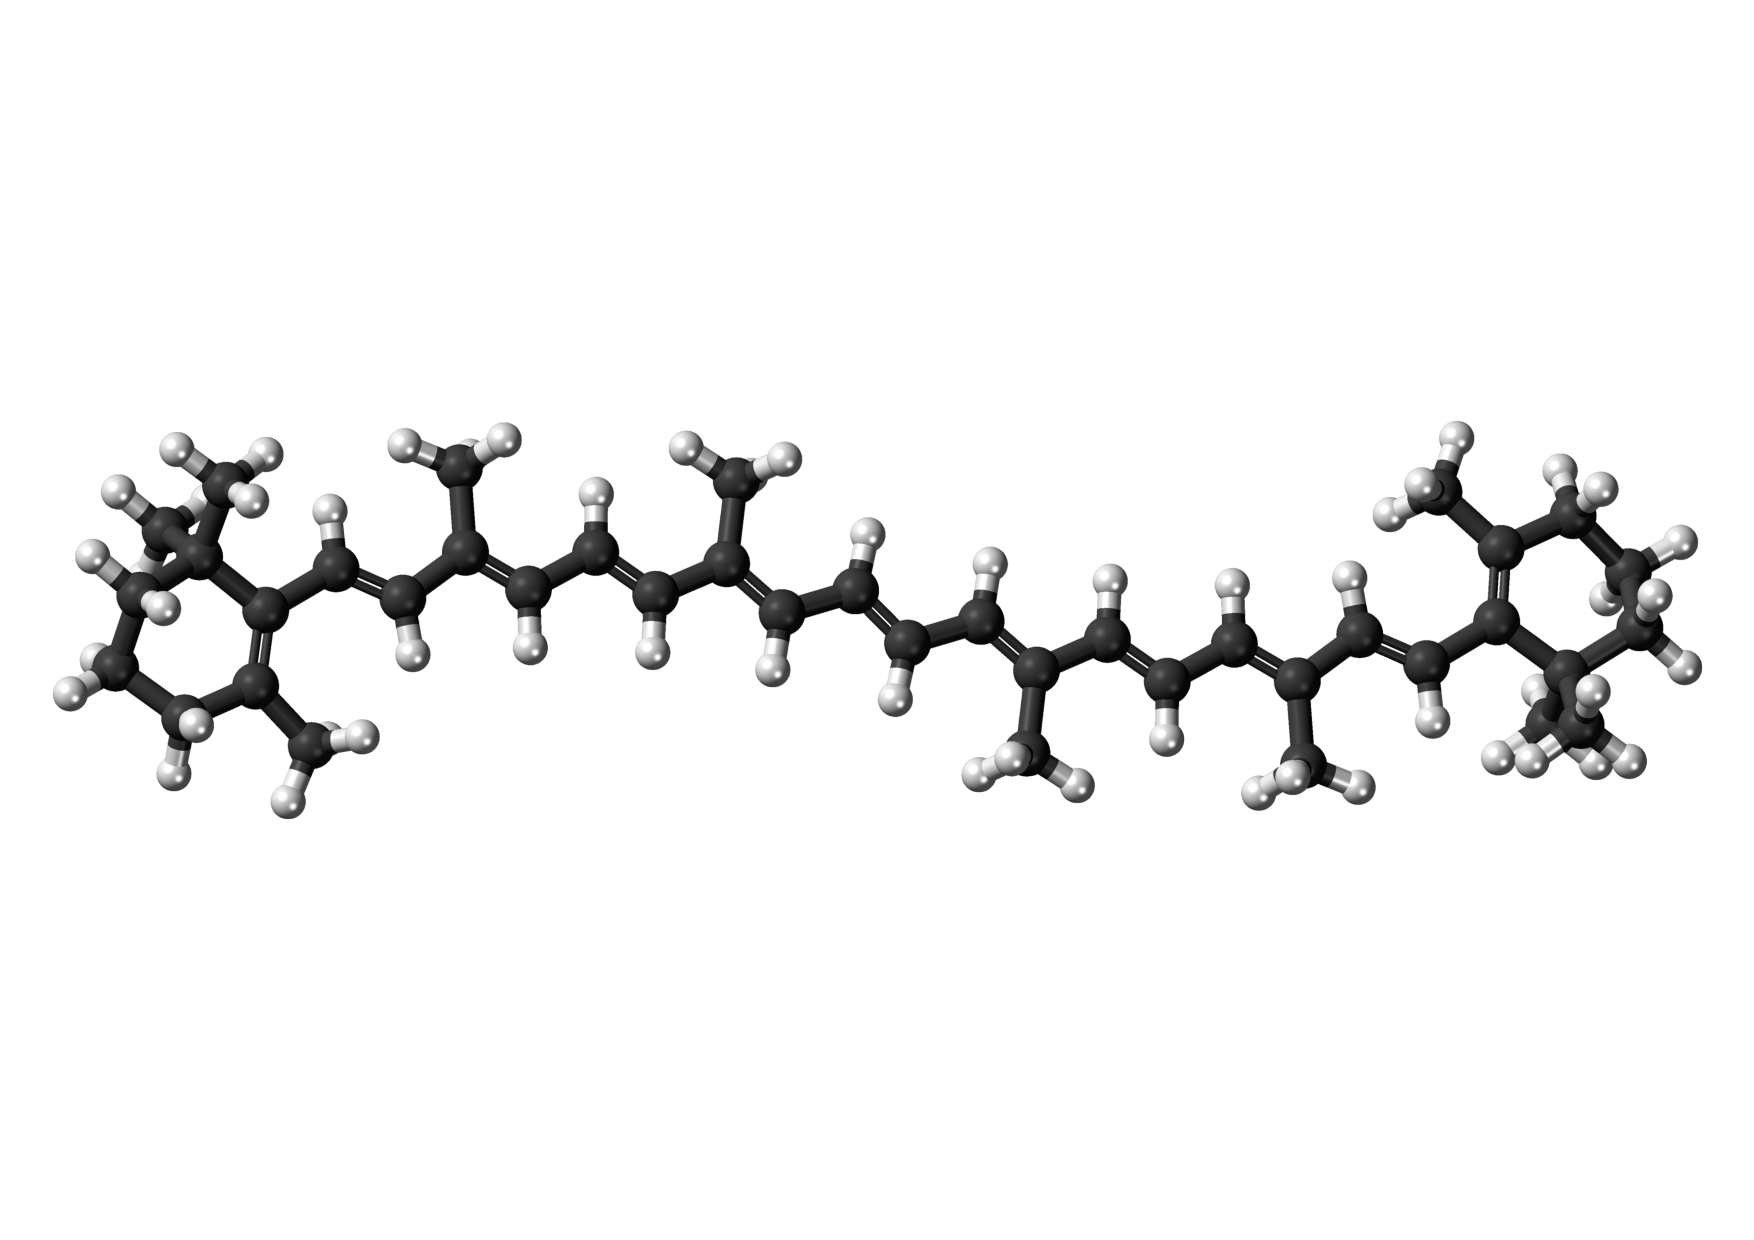
\includegraphics[scale=0.3, clip, viewport = 0 150 900 430]{figures/beta-carotene.pdf}
    \end{center}
    }
\end{frame}

\begin{frame}
    \frametitle{Density Functional Theory}
    \centering
    Dramatically reduce the dimensionality
    \begin{equation}
	\nonumber
	\rho(\boldsymbol{r}_1) = N \int |\psi(\boldsymbol{r}_1, \boldsymbol{r}_2,\dots,
	\boldsymbol{r}_N)|^2 d\boldsymbol{r}_2\cdots d\boldsymbol{r}_N
    \end{equation}
    \ \\
    \ \\
    \ \\
    \pause
    Energy expressed as functional of the density
    \begin{equation}
	\nonumber
	E[\rho] = T_s[\rho] + V_{ne}[\rho] + J[\rho] + E_{xc}[\rho]
    \end{equation}
    \ \\
    \ \\
    \ \\
    \begin{columns}
    \begin{column}{.50\textwidth}
    \centering
    \pause
    \textbf{Energy expressions}
    \begin{align}
	\nonumber
	V_{ne}[\rho]	&= \int \rho(\boldsymbol{r})v_{nuc}(\boldsymbol{r})d\boldsymbol{r}\\
	\nonumber
			&\\
	\nonumber
	J[\rho] &= \frac{1}{2} \int \rho(\boldsymbol{r})v_{el}(\boldsymbol{r})d\boldsymbol{r}\\
	\nonumber
			&\\
	\nonumber
	E_{xc}[\rho]	&= \int F_{xc}(\rho) d\boldsymbol{r}
    \end{align}
    \end{column}
    \begin{column}{.50\textwidth}
    \centering
    \pause
    \textbf{Potentials}
    \begin{align}
	\nonumber
	v_{nuc}(\boldsymbol{r}) &= -\sum_I\frac{Z_I}{|\boldsymbol{r}-\boldsymbol{R}_I|}\\
	\nonumber
			&\\
	\nonumber
	v_{el}(\boldsymbol{r}) &= 
	    \int \frac{\rho(\boldsymbol{r}')}{4\pi|\boldsymbol{r}-\boldsymbol{r}'|} d\boldsymbol{r}'\\
	\nonumber
			&\\
	\nonumber
	v_{xc}(\boldsymbol{r}) &= \frac{\delta E_{xc}[\rho]}{\delta\rho}
    \end{align}
    \end{column}
    \end{columns}    
\end{frame}

\begin{frame}
    \frametitle{Kohn-Sham DFT}
    \centering
    Express density through one-electron orbitals
    \begin{equation}
	\nonumber
	\rho(\boldsymbol{r}) = \sum_i |\phi_i(\boldsymbol{r})|^2
    \end{equation}
    \ \\
    \ \\
    \ \\
    \ \\
    \pause
    \begin{columns}
    \begin{column}{.50\textwidth}
    \centering
    Kinetic energy
    \begin{equation}
	\nonumber
	T_s[\rho] = -\sum_i \frac{1}{2}\nabla^2\phi_i(\boldsymbol{r})
    \end{equation}
    \end{column}
    \begin{column}{.50\textwidth}
    \centering
    Effective potential
    \begin{equation}
	\nonumber
	v_{eff}(\boldsymbol{r}) = v_{nuc}(\boldsymbol{r}) + v_{el}(\boldsymbol{r}) + v_{xc}(\boldsymbol{r})
    \end{equation}
    \end{column}
    \end{columns}
    \ \\
    \ \\
    \ \\
    \ \\
    \pause
    \centering
    \textbf{The Kohn-Sham equations}
    \begin{equation}
	\nonumber
	\left[-\frac{1}{2}\nabla^2 + v_{eff}(\boldsymbol{r})\right]\phi_i(\boldsymbol{r}) = 
	\epsilon_i\phi_i(\boldsymbol{r})
    \end{equation}
\end{frame}

\begin{frame}
    \frametitle{Variation principle}
    \begin{columns}
    \begin{column}{.50\textwidth}
    \centering
    \textbf{Solving the Kohn-Sham equations}
    \begin{equation}
	\nonumber
	\bigg[-\frac{1}{2}\nabla^2 + \hat{V}\bigg]\phi_i(r) = \epsilon_i \phi_i(r)
    \end{equation}
    \end{column}
    \begin{column}{.50\textwidth}
    \centering
    \textbf{Equivalent of minimizing the energy}
    \begin{equation}
        E_0 = \mymin{\rho}\ E[\rho]
    \end{equation}
    \end{column}
    \end{columns}

    \vspace{5mm}


\end{frame}

\begin{frame}
    \frametitle{The Kohn-Sham equations}
\end{frame}

\begin{frame}
    \frametitle{Density Functional Approximations}
\end{frame}

\begin{frame}
    \frametitle{Computational chemistry}
    \begin{center}
    \only<1>{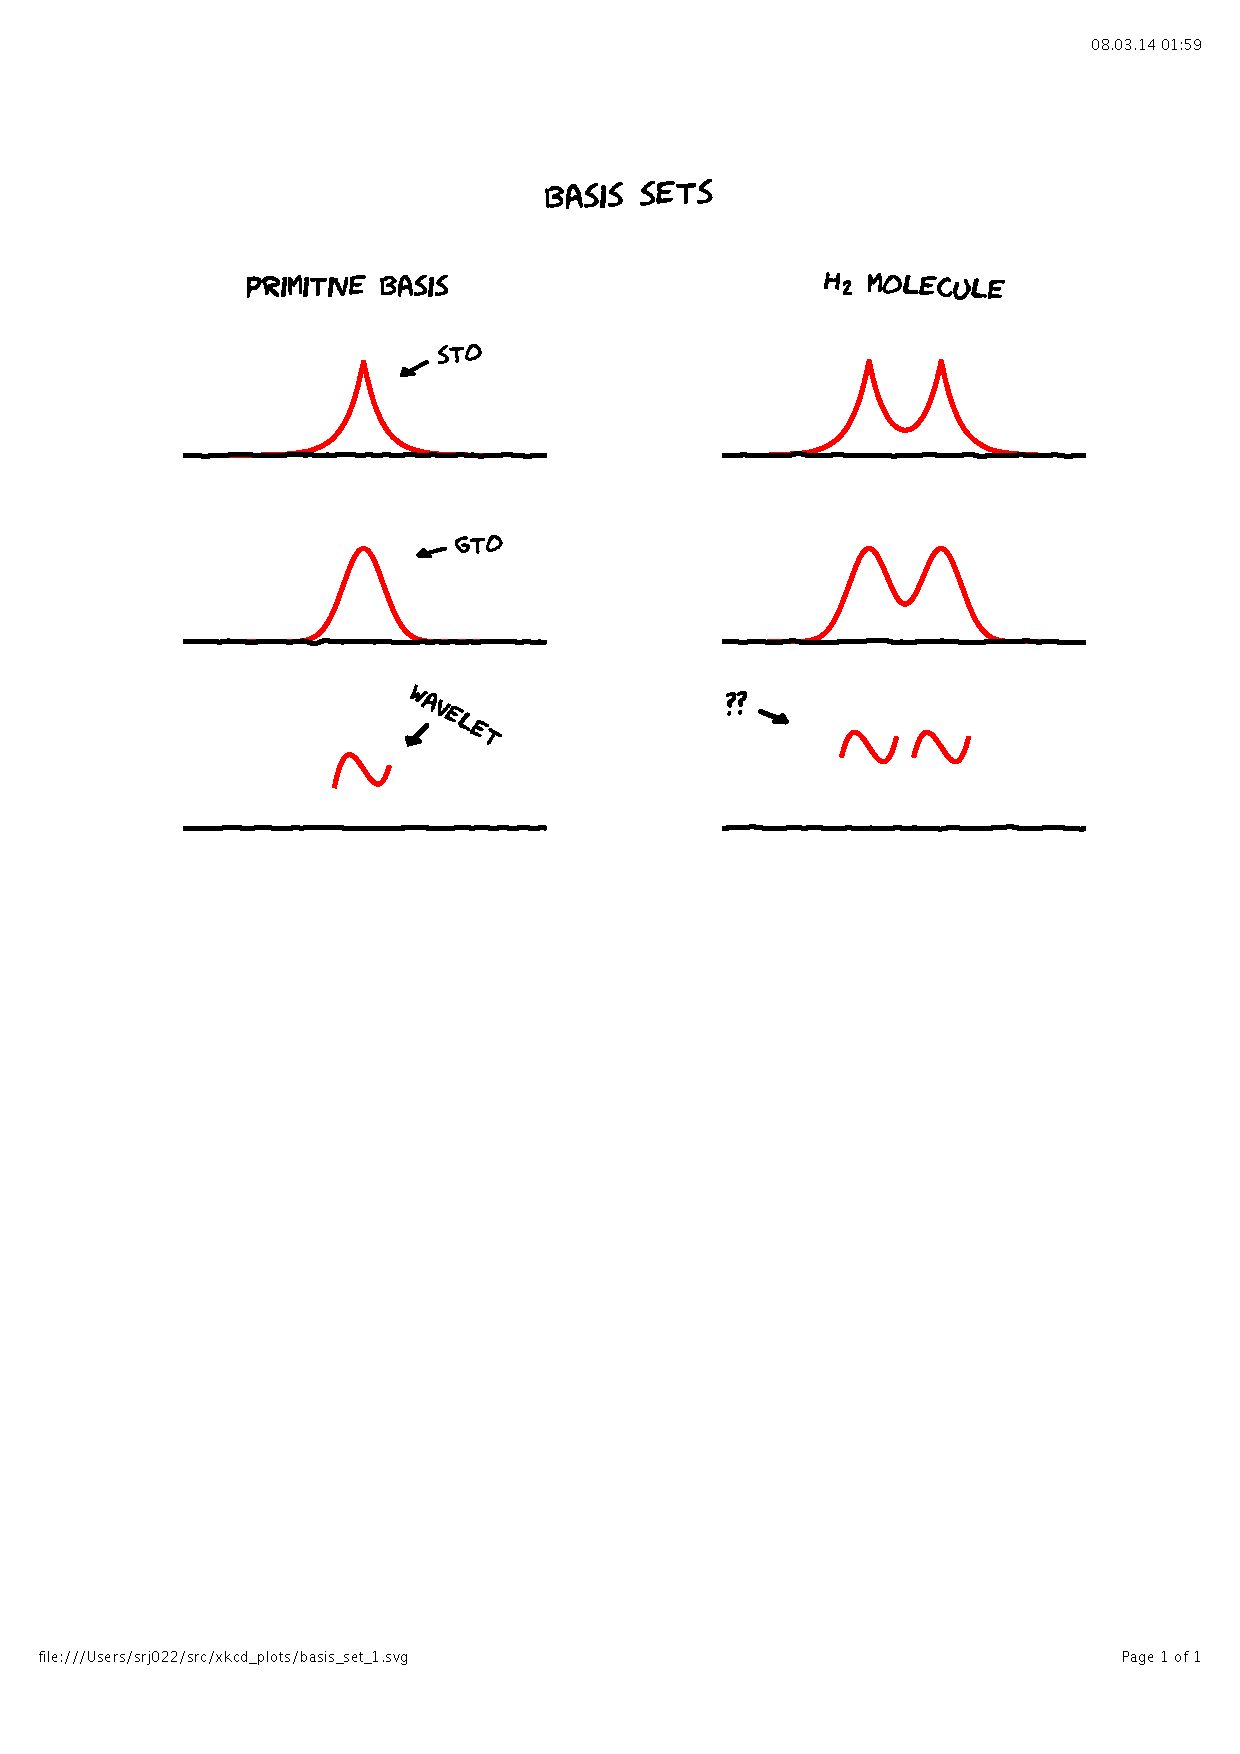
\includegraphics[scale=0.5, clip, viewport = 50 300 550 800]{figures/basis_set_1.pdf}}
    \only<2>{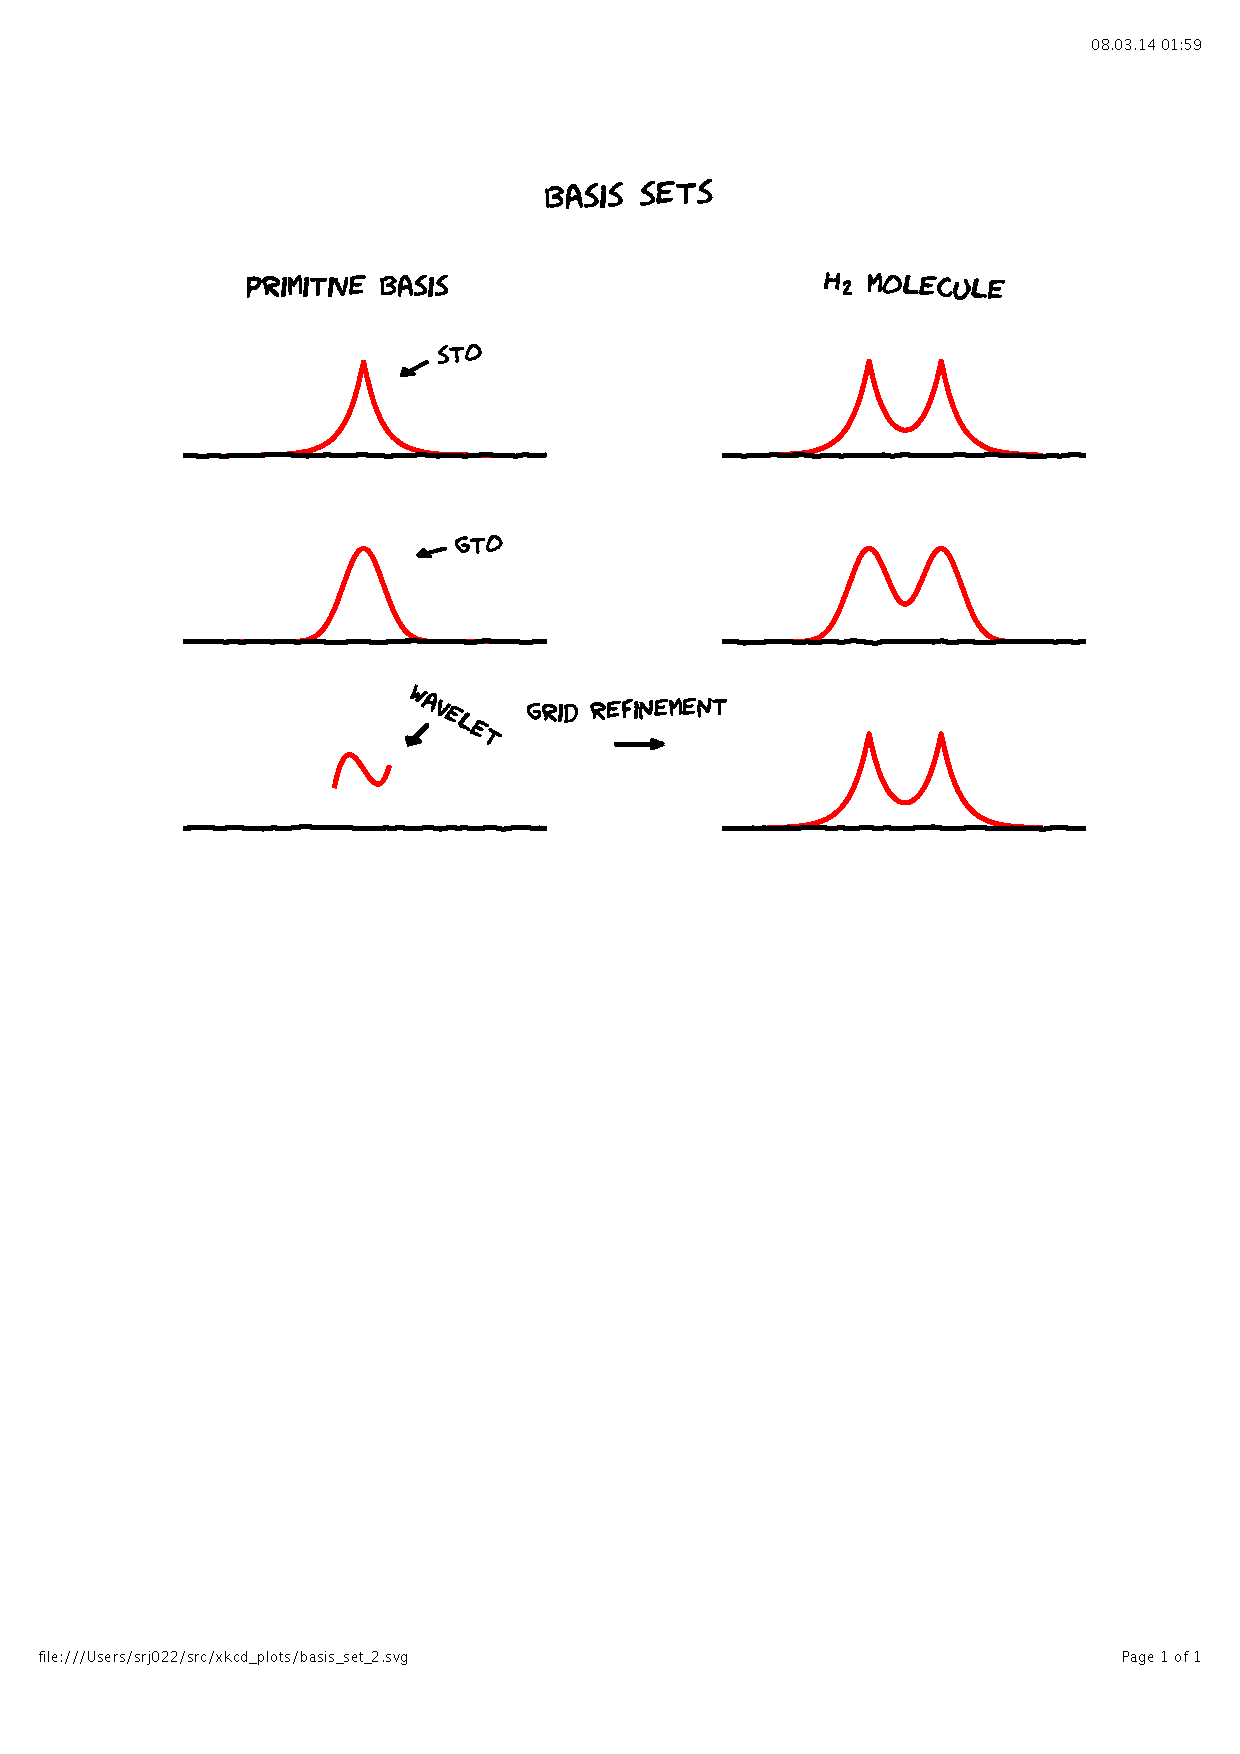
\includegraphics[scale=0.5, clip, viewport = 50 300 550 800]{figures/basis_set_2.pdf}}
    \end{center}
\end{frame}

\begin{frame}
    \frametitle{Integral formulation SCF}
    \centering
    \textbf{SCF equations}
    \begin{equation}
	\nonumber
	\bigg[-\frac{1}{2}\nabla^2 + \hat{V}\bigg]\phi_i(r) = \epsilon_i \phi_i(r)
    \end{equation}

    \vspace{5mm}

    \textbf{Rewrite using} $\mu_i^2 = -2\epsilon_i$
    \begin{align}
	\nonumber
	\Big[-\nabla^2 + \mu_i^2\Big]\phi_i(r) =&\ -2\hat{V}\phi_i(r)\\
	\nonumber
	\phi_i(r) =&-2\Big[-\nabla^2 + \mu_i^2\Big]^{-1}\hat{V}\phi_i(r)\\
	\nonumber
	\phi_i =&-2\hat{G}_{\mu_i}\Big[\hat{V}\phi_i\Big]
    \end{align}

    \vspace{5mm}

    \textbf{Bound-State Helmholtz operator}
    \begin{equation}
	\nonumber
	\hat{G}_{\mu_i}f(r) = \int \frac{e^{-\mu_i |r-r'|}}{4\pi|r-r'|}f(r')dr'
    \end{equation}

    \vspace{5mm}

    \centering
    \tiny
    MH Kalos,
    {\it Phys. Rev.}, 
    \textbf{128(4)},
    1791 (1962)\\
    RJ Harrison, GI Fann, T Yanai, Z Gan and G Beylkin,
    {\it J. Chem. Phys.}, 
    \textbf{121},
    11587 (2004)
\end{frame}

\begin{frame}
    \frametitle{Total energy calculation}
    \centering
    \textbf{Kohn-Sham energy expression}
    \begin{equation}
        \nonumber
        E[\rho] = T_s[\rho] + V_{en}[\rho] + J[\rho] + E_{xc}[\rho]
    \end{equation}

    \vspace{3mm}

    \textbf{Closed-shell system}
    \begin{equation}
        \nonumber
        E = \sum_i^{N/2} 2\langle \phi_i|\hat{T}|\phi_i \rangle
	    + \int \rho(r)v_{nuc}(r) \ud r
	    + \frac{1}{2} \int \rho(r)v_{el}(r) \ud r
	    + \int F_{xc} \ud r
    \end{equation}

    \vspace{3mm}

    \textbf{Sum of orbital energies}
    \begin{equation}
        \nonumber
        \sum_i^{N/2} 2\epsilon_i 
	    = \sum_i^{N/2} 2\langle\phi_i|\hat{T} + \hat{V}|\phi_i\rangle
	    = \sum_i^{N/2} 2\langle\phi_i|\hat{T}|\phi_i\rangle
	        + \int \rho(r)\Big[v_{nuc}(r)+v_{el}(r)+v_{xc}(r)\Big] \ud r
    \end{equation}

    \vspace{3mm}

    \textbf{Alternative expression}
    \begin{equation}
        \nonumber
        E = 2 \sum_i^{N/2} \epsilon_i - \frac{1}{2} \int \rho(r)v_{el}(r) \ud r
	    + \int F_{xc} \ud r - \int \rho(r)v_{xc}(r) \ud r
    \end{equation}
\end{frame}

\begin{frame}
    \centering
    \Large{Part II:}
    
    \vspace{5mm}

    \centering
    \textbf{\Large{Iterative solution algorithms}}
\end{frame}

\begin{frame}
    \frametitle{One-electron systems}
    \centering
    \textbf{Potential operator}
    \begin{equation}
	\nonumber
	\hat{V} = v_{nuc}(r) = -\sum_I\frac{Z_I}{|r-R_I|}
    \end{equation}

    \vspace{5mm}

    \textbf{Smoothed nuclear potential}
    \begin{align}
	\nonumber
	\frac{1}{r} &\approx \frac{erf(r)}{r} +
	\frac{1}{3\sqrt{\pi}}\big(e^{-r^2}+16e^{-4r^2}\big)
    \end{align}

    \vspace{5mm}

    \textbf{One-electron Schr\"{o}dinger equation}
    \begin{equation}
        \nonumber
        \Big[-\frac{1}{2}\nabla^2 + \hat{V}\Big]\psi(r) = E \psi(r)
    \end{equation}

    \vspace{1mm}

    \begin{equation}
        \nonumber
        \psi = -2\hat{G}_\mu \Big[\hat{V} \psi \Big]
    \end{equation}

    \vspace{5mm}

    \centering
    \tiny
    RJ Harrison, GI Fann, T Yanai, Z Gan and G Beylkin,
    {\it J. Chem. Phys.}, 
    \textbf{121},
    11587 (2004)
\end{frame}

\begin{frame}
    \frametitle{One-electron algorithm}
    \centering
    \textbf{Power iteration of the BSH operator}
    \begin{equation}
	\nonumber
	\psi^{n+1} = -2G^n\Big[\hat{V} \psi^n\Big]
    \end{equation}

    \vspace{3mm}

    \textbf{Finding roots of the residual}
    \begin{equation}
	\nonumber
	f(\psi) = -2G^n\big[\hat{V} \psi\big] -\psi
    \end{equation}

    \vspace{3mm}

    \textbf{Newton's method}
    \begin{equation}
	\nonumber
	\psi^{n+1} = \psi^n - \Big[J(\psi^n)\Big]^{-1} f(\psi^n)
    \end{equation}

    \begin{equation}
	\nonumber
	\psi^{n+1} = \psi^n - \Big[J(\psi^n)\Big]^{-1}
	\bigg(-2G^n\Big[\hat{V}\psi^n\Big] - \psi^n\bigg)
    \end{equation}

    \vspace{3mm}

    So the direct power iteration is an "inexact" Newton method\\
    where we approximate the Jacobian $J(\psi^n) \approx -1$.
\end{frame}

\begin{frame}
    \frametitle{One-electron algorithm}
    \begin{columns}
    \begin{column}{.50\textwidth}
    \centering
    \textbf{Initialize BSH operator} $\hat{G}^n$
    \begin{equation}
        \nonumber
        \mu^n = \sqrt{-2E^n}
    \end{equation}
    \end{column}

    \begin{column}{.50\textwidth}
    \centering
    \textbf{Power iteration}
    \begin{equation}
	\nonumber
	\tilde{\psi}^{n+1} = -2\hat{G}^n \Big[ \hat{V} \psi^n \Big]
    \end{equation}
    \end{column}
    \end{columns}

    \vspace{5mm}

    \begin{columns}
    \begin{column}{.50\textwidth}
    \centering
    \textbf{Orbital update}
    \begin{equation}
	\nonumber
	\Delta\psi^n = \frac{\tilde{\psi}^{n+1}}{\|\tilde{\psi}^{n+1}\|} - \psi^n
    \end{equation}
    \end{column}

    \begin{column}{.50\textwidth}
    \centering
    \textbf{Energy update}
    \begin{equation}
	\nonumber
	\Delta E^n =
        \frac{\langle\tilde{\psi}^{n+1}|\hat{V}|\Delta\tilde{\psi}^n\rangle}
        {\langle\tilde{\psi}^{n+1}|\tilde{\psi}^{n+1}\rangle}
    \end{equation}
    \end{column}
    \end{columns}

    \vspace{10mm}

    \centering
    \textbf{Update wavefunction and energy}
    \begin{align}
	\nonumber
        \psi^{n+1}  &= \psi^n + \Delta \psi^n\\
	\nonumber
        E^{n+1}     &= E^n + \Delta E^n
    \end{align}
\end{frame}

\begin{frame}
    \frametitle{Energy update}
    \centering
    \textbf{Using the relation}
    \begin{equation}
        \nonumber
        -2\hat{G}^n = \big(\hat{T} - E^n\big)^{-1}
    \end{equation}

    \vspace{5mm}

    \begin{align}
        \tilde{E}^{n+1}
        \nonumber
        &=	\langle\tilde{\psi}^{n+1}| \hat{T}+\hat{V} | \tilde{\psi}^{n+1}\rangle\\
        \nonumber
        &=	\langle\tilde{\psi}^{n+1}|  \hat{T} - E^n  | \tilde{\psi}^{n+1}\rangle
        +	\langle\tilde{\psi}^{n+1}|  E^n + \hat{V}  | \tilde{\psi}^{n+1}\rangle\\
        \nonumber
        &=	\langle\tilde{\psi}^{n+1}|  \hat{T} - E^n  | 
	        -2\hat{G}^n\big[\hat{V}\psi^n\big]\rangle
        +	\langle\tilde{\psi}^{n+1}| E^n + \hat{V} |\tilde{\psi}^{n+1}\rangle\\
        \nonumber
        &= -\langle\tilde{\psi}^{n+1}| \hat{V} |\psi^{n}\rangle
        +	\langle\tilde{\psi}^{n+1}| E^n + \hat{V} |\tilde{\psi}^{n+1}\rangle\\
        \nonumber
        &= E^{n}\langle\tilde{\psi}^{n+1}|\tilde{\psi}^{n+1}\rangle + 
	    \langle\tilde{\psi}^{n+1}| \hat{V} |\Delta\tilde{\psi}^{n}\rangle
    \end{align}

    \vspace{8mm}

    \centering
    Energy expression without the kinetic operator
    \begin{equation}
        \nonumber
        E^{n+1} = E^{n} + 
        \frac{\langle\tilde{\psi}^{n+1}| \hat{V} |\Delta\tilde{\psi}^{n}\rangle}
        {\langle\tilde{\psi}^{n+1}|\tilde{\psi}^{n+1}\rangle}
    \end{equation}
\end{frame}

\begin{frame}
    \frametitle{Hydrogen atom}
    \begin{center}
	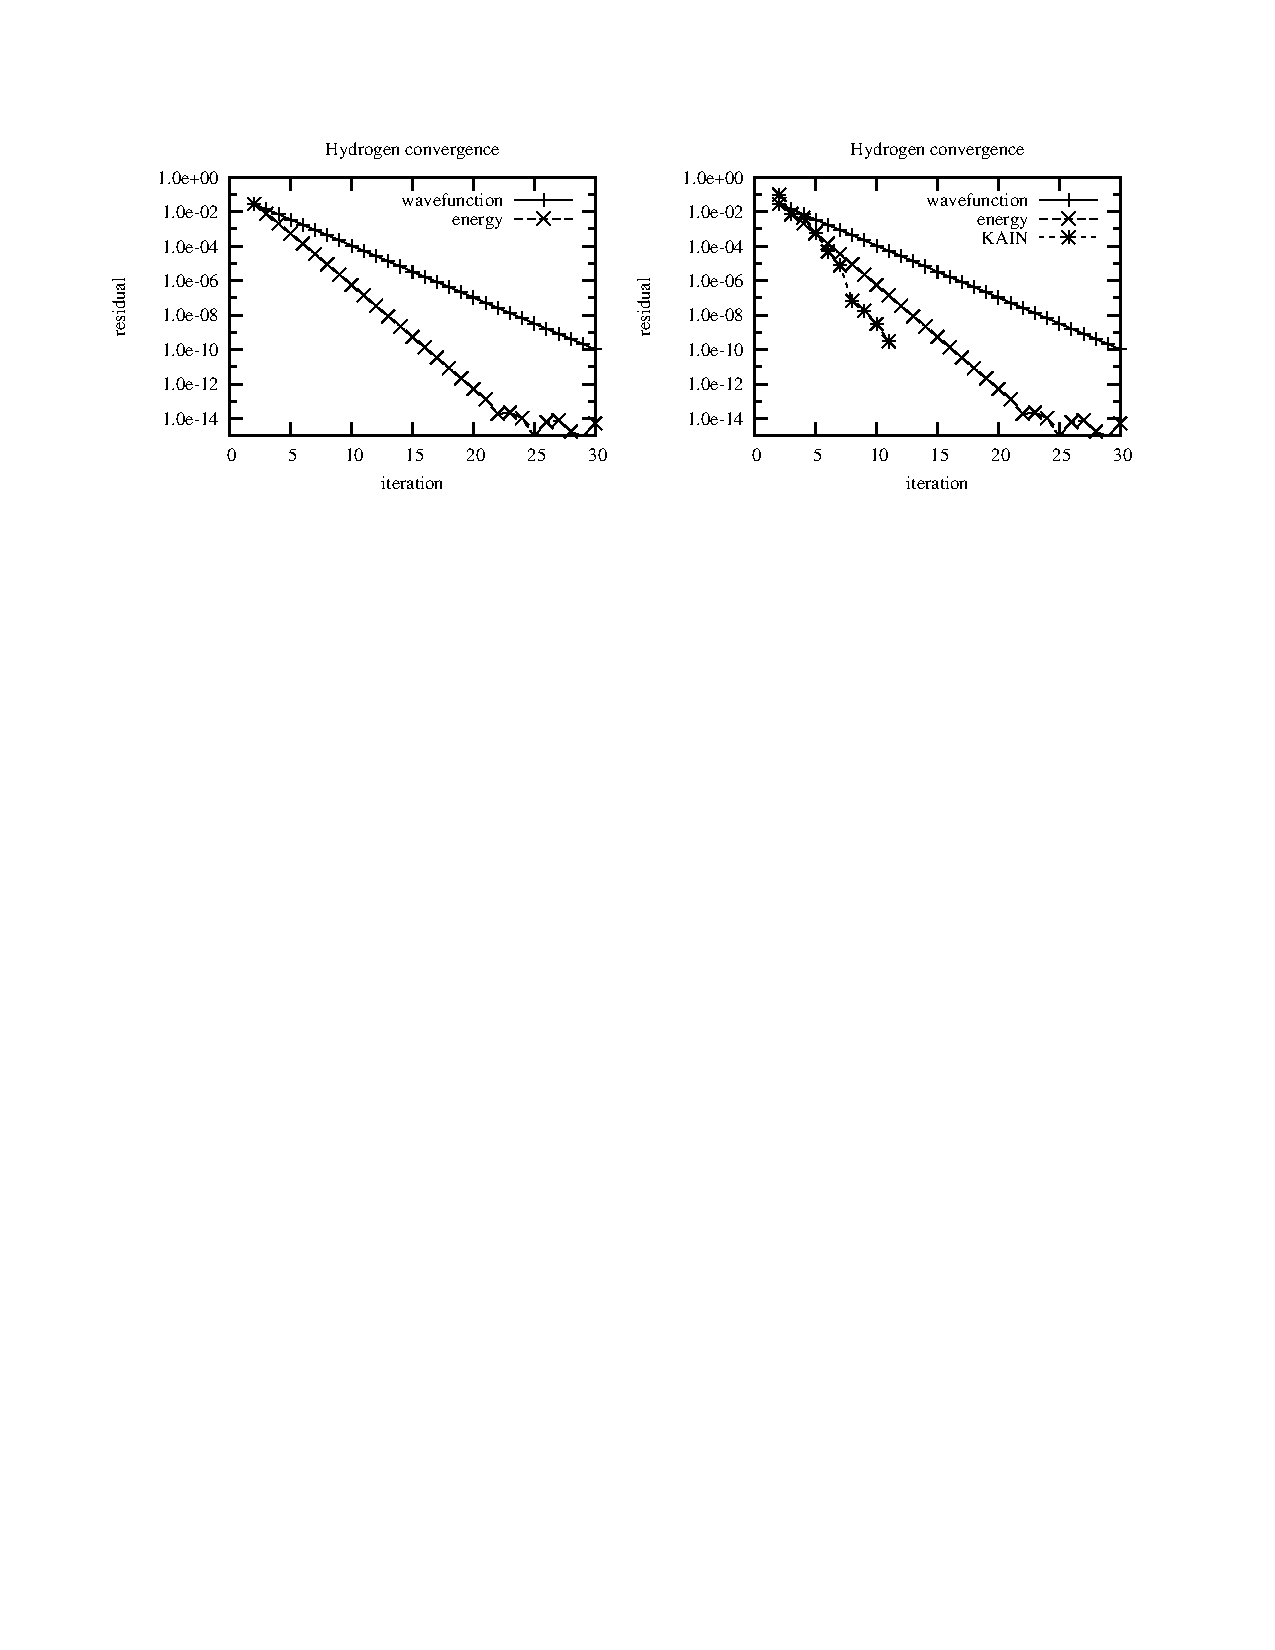
\includegraphics[scale=1.0, clip, viewport = 50 550 300 730]{figures/h_convergence.pdf}
    \end{center}
\end{frame}

\begin{frame}
    \frametitle{Krylov subspace Accelerated Inexact Newton (KAIN)}
    \begin{columns}
    \begin{column}[b]{0.5\textwidth}
    \centering
    \textbf{Wavefunction history}
    \begin{equation}
	\nonumber
	\psi^0, \psi^1, \dots, \psi^n
    \end{equation}
    \end{column}
    \begin{column}[b]{0.5\textwidth}
    \centering
    \textbf{Residual history}
    \begin{equation}
	\nonumber
	f(\psi^0), f(\psi^1), \dots, f(\psi^n)
    \end{equation}
    \end{column}
    \end{columns}

    \vspace{5mm}

    \centering
    \textbf{Used to find a better approximation to the Jacobian}

    \vspace{10mm}

    The new iterative step is then expanded in the Krylov subspace
    \begin{equation}
	\nonumber
	\delta\psi^n = \sum_i c_i\Big(\psi^i-\psi^n\Big) - 
	\sum_i c_i\Big(f(\psi^i) - f(\psi^n)\Big) - f(\psi^n)
    \end{equation}

    \vspace{5mm}

    by solving the linear system $Ac = b$
    \begin{align}
	\nonumber
	A_{ij} &= \langle\psi^n-\psi^i|f(\psi^n) - f(\psi^j)\rangle\\
	\nonumber
	b_{i}  &= \langle\psi^n-\psi^i|f(\psi^n)\rangle
    \end{align}

    \vspace{5mm}

    \centering
    \tiny
    RJ Harrison,
    {\it J. Comput. Chem.}, 
    \textbf{25(3)},
    328 (2004)
\end{frame}

\begin{frame}
    \frametitle{One-electron algorithm}

    \begin{columns}
    \begin{column}{.50\textwidth}
    \centering
    \textbf{Initialize BSH operator} $\hat{G}^n$
    \begin{equation}
        \nonumber
        \mu^n = \sqrt{-2E^n}
    \end{equation}
    \end{column}

    \begin{column}{.50\textwidth}
    \centering
    \textbf{Power iteration}
    \begin{equation}
	\nonumber
	\tilde{\psi}^{n+1} = -2\hat{G}^n \Big[ \hat{V} \psi^n \Big]
    \end{equation}
    \end{column}
    \end{columns}

    \vspace{5mm}

    \begin{columns}
    \begin{column}{.50\textwidth}
    \centering
    \textbf{Orbital update}
    \begin{equation}
	\nonumber
	\Delta\psi^n = \frac{\tilde{\psi}^{n+1}}{\|\tilde{\psi}^{n+1}\|} - \psi^n
    \end{equation}
    \end{column}

    \begin{column}{.50\textwidth}
    \centering
    \textbf{Energy update}
    \begin{equation}
	\nonumber
	\Delta E^n =
        \frac{\langle\tilde{\psi}^{n+1}|\hat{V}|\Delta\tilde{\psi}^n\rangle}
        {\langle\tilde{\psi}^{n+1}|\tilde{\psi}^{n+1}\rangle}
    \end{equation}
    \end{column}
    \end{columns}

    \vspace{5mm}

    \centering
    \textbf{KAIN update}
    \begin{equation}
	\nonumber
        \left(
        \begin{matrix}
        \delta \psi\\
        \delta E
        \end{matrix}
        \right)^{n+1}
        \longleftarrow
        \left(
        \begin{matrix}
        \psi\\
        E
        \end{matrix}
        \right)^n
        ,
        \left(
        \begin{matrix}
        \Delta \psi\\
        \Delta E
        \end{matrix}
        \right)^n
    \end{equation}

    \vspace{5mm}

    \textbf{Update wavefunction and energy}
    \begin{align}
	\nonumber
        \psi^{n+1}  &= \psi^n + \delta \psi^n\\
	\nonumber
        E^{n+1}     &= E^n + \delta E^n
    \end{align}
\end{frame}

\begin{frame}
    \frametitle{Hydrogen atom}
    \begin{center}
	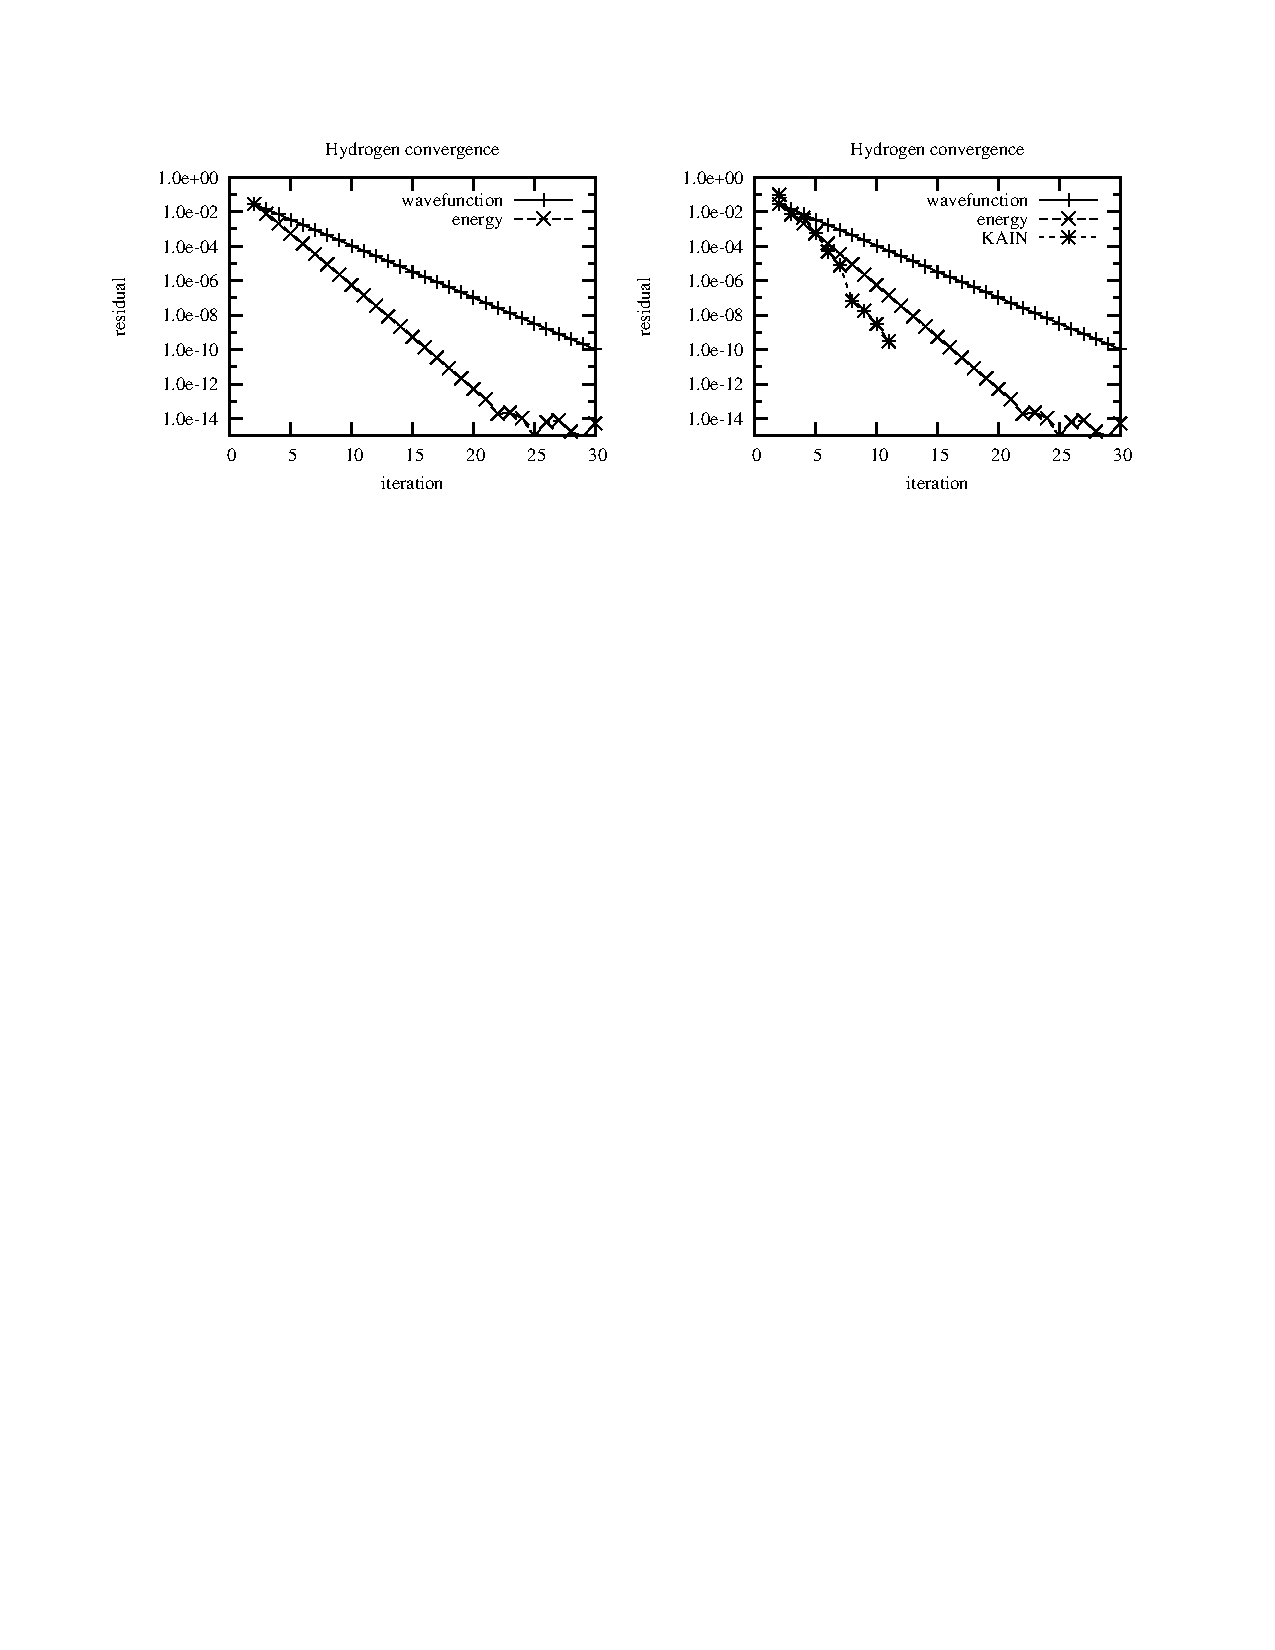
\includegraphics[scale=1.0, clip, viewport = 300 550 560 740]{figures/h_convergence.pdf}
    \end{center}
\end{frame}

\begin{frame}
    \frametitle{Many-electron systems}
    \centering
    \textbf{Potential operator}
    \begin{equation}
        \nonumber
        \hat{V} = v_{nuc}(r) + v_{el}(r) + v_{xc}(r) - \hat{K}
    \end{equation}

    \vspace{10mm}

    \begin{columns}
    \begin{column}[b]{0.5\textwidth}
    \centering
    \textbf{Classical nuclear}
    \begin{equation}
        \nonumber
	v_{nuc}(r) = -\sum_I\frac{Z_I}{|r-R_I|}
    \end{equation}
    \end{column}

    \begin{column}[b]{0.5\textwidth}
    \centering
    \textbf{Classical Coulomb}
    \begin{equation}
        \nonumber
        v_{el}(r) = \int \frac{\rho(r')}{4\pi|r-r'|} \ud r'
    \end{equation}
    \end{column}
    \end{columns}

    \vspace{5mm}

    \begin{columns}
    \begin{column}[b]{0.5\textwidth}
    \centering
    \textbf{Exchange-Correlation}
    \begin{equation}
        \nonumber
        v_{xc}(r)
        = \frac{\delta E_{xc}}{\delta \rho}
        = \frac{\partial F_{xc}}{\partial \rho} - \nabla \cdot \frac{\partial F_{xc}}{\partial \nabla\rho}
    \end{equation}
    \end{column}

    \begin{column}[b]{0.5\textwidth}
    \centering
    \textbf{Hartree-Fock exchange}
    \begin{equation}
        \nonumber
        \hat{K}\phi_p(r) = \sum_i \phi_i(r) \int \frac{\phi_i^\dagger(r')\phi_p(r')}{4\pi|r-r'|} \ud r'
    \end{equation}
    \end{column}
    \end{columns}
\end{frame}

\begin{frame}
    \frametitle{Orthonormalization}
    \centering
    \textbf{Straightforward iteration of the Kohn-Sham equations}
    \begin{equation}
        \nonumber
        \tilde{\phi}_i^{n+1} = -2\hat{G}^n \bigg[\hat{V}^n\phi_i^n\bigg]
    \end{equation}
    \textbf{brings all orbitals to the lowest energy eigenfunction}
    
    \vspace{15mm}

    \textbf{Orthonormality must be imposed}
    \begin{equation}
        \nonumber
        \tilde{S}_{ij} = \langle\tilde{\phi}_i|\tilde{\phi}_j\rangle = \delta_{ij}
    \end{equation}

    \vspace{5mm}

    \begin{columns}
    \begin{column}[b]{0.5\linewidth}
    \centering
    \textbf{Gram-Schmidt}
    \begin{equation}
	\nonumber
	\phi_i = \Big(1 - \sum_{j<i}|\phi_j\rangle\langle\phi_j|\Big)\tilde{\phi}_i
    \end{equation}
    \end{column}

    \begin{column}[b]{0.5\linewidth}
    \centering
    \textbf{L\"{o}wdin orthonormalization}
    \begin{equation}
	\nonumber
	\phi_i = \sum_j \tilde{S}_{ij}^{-1/2}\tilde{\phi}_j
    \end{equation}
    \end{column}
    \end{columns}
\end{frame}

\begin{frame}
    \frametitle{Canonical orbitals}
    Derive non-canonical equations w/lambda
    Define Fock matrix
    Diagonalize Fock matrix
\end{frame}

\begin{frame}
    \frametitle{Localized orbitals}
    \centering
    Total energy invariant under unitary transformations among occupied orbitals
    \begin{equation}
	\nonumber
	\phi_i = \sum_j L_{ij} \phi_i, \qquad \qquad L^\ast L = LL^\ast = I
    \end{equation}

    \begin{columns}
    \begin{column}[b]{0.48\linewidth}
    \centering
    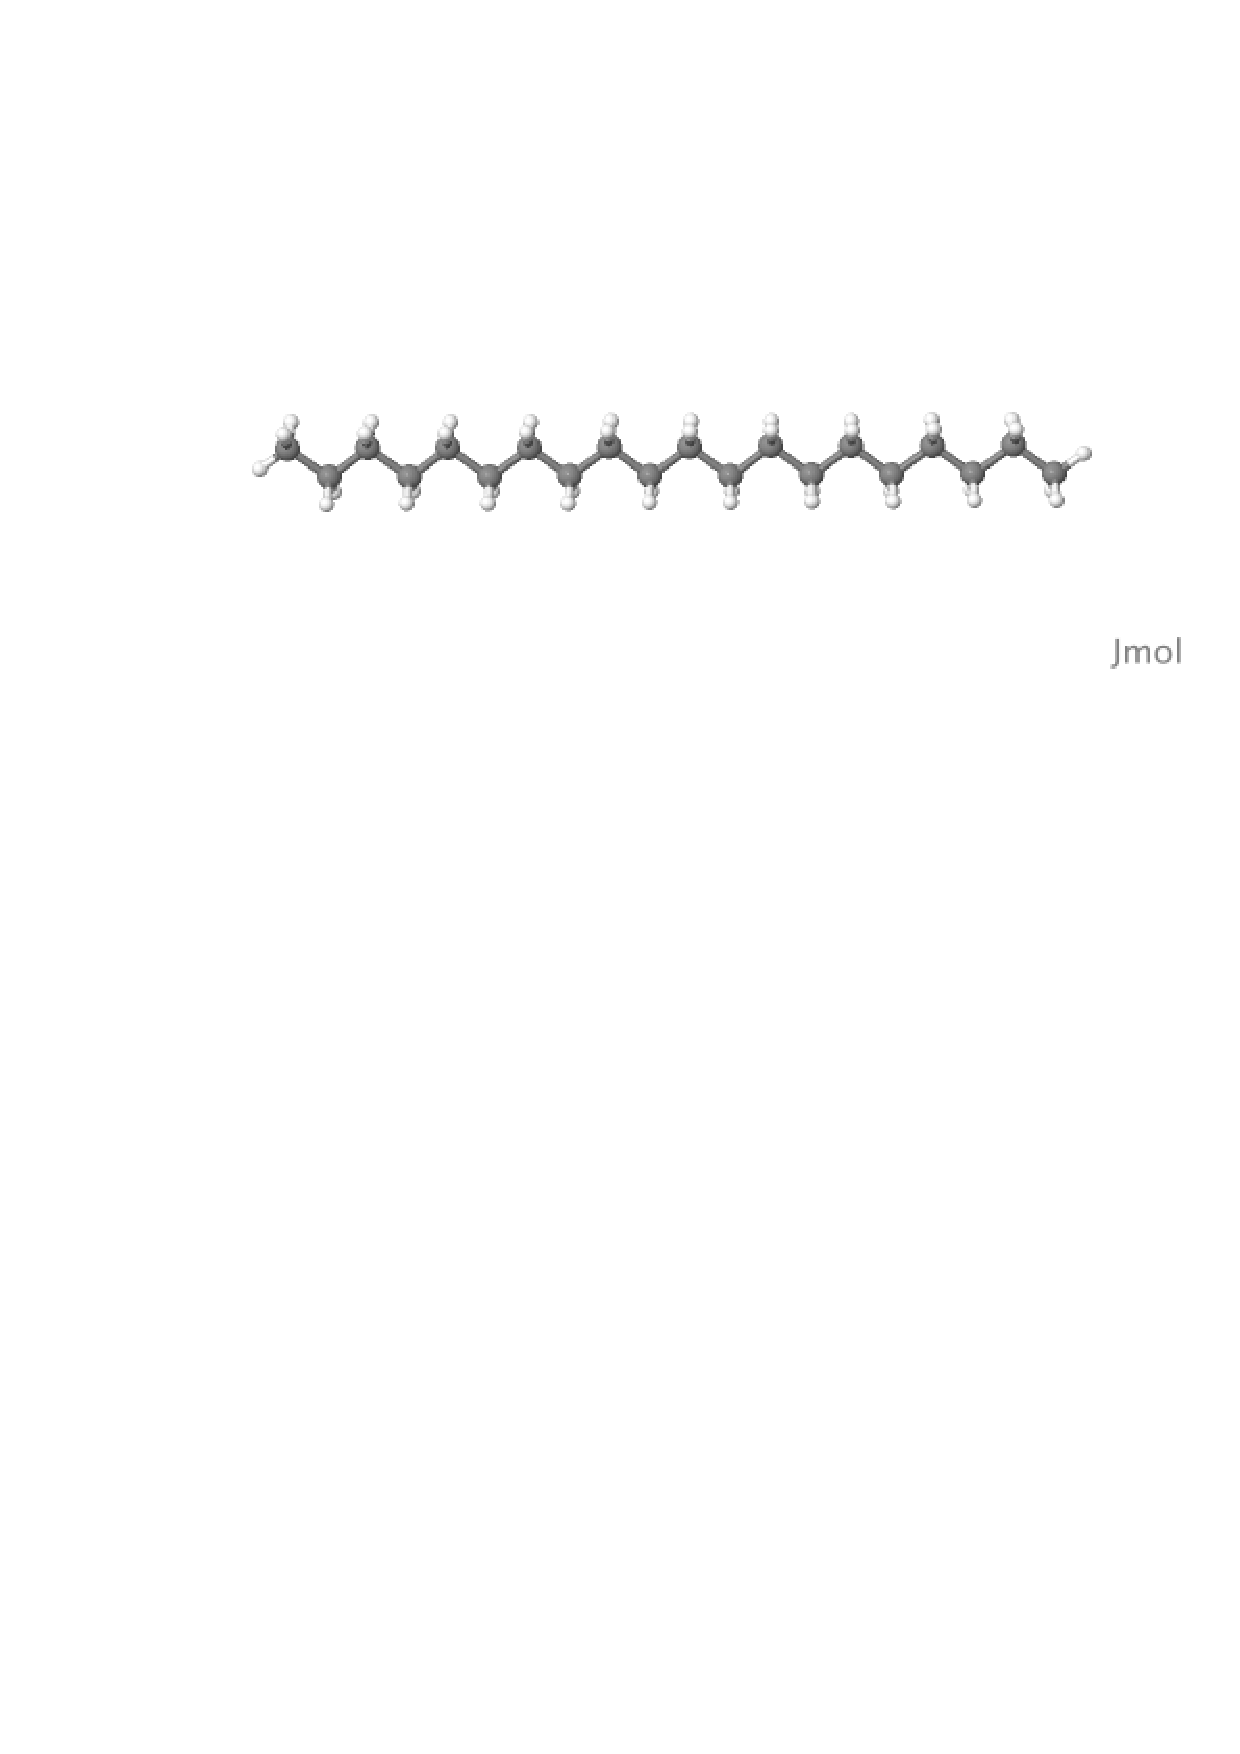
\includegraphics[scale=0.25, clip, viewport = 80 560 600 700]{figures/alkane.pdf}\\
    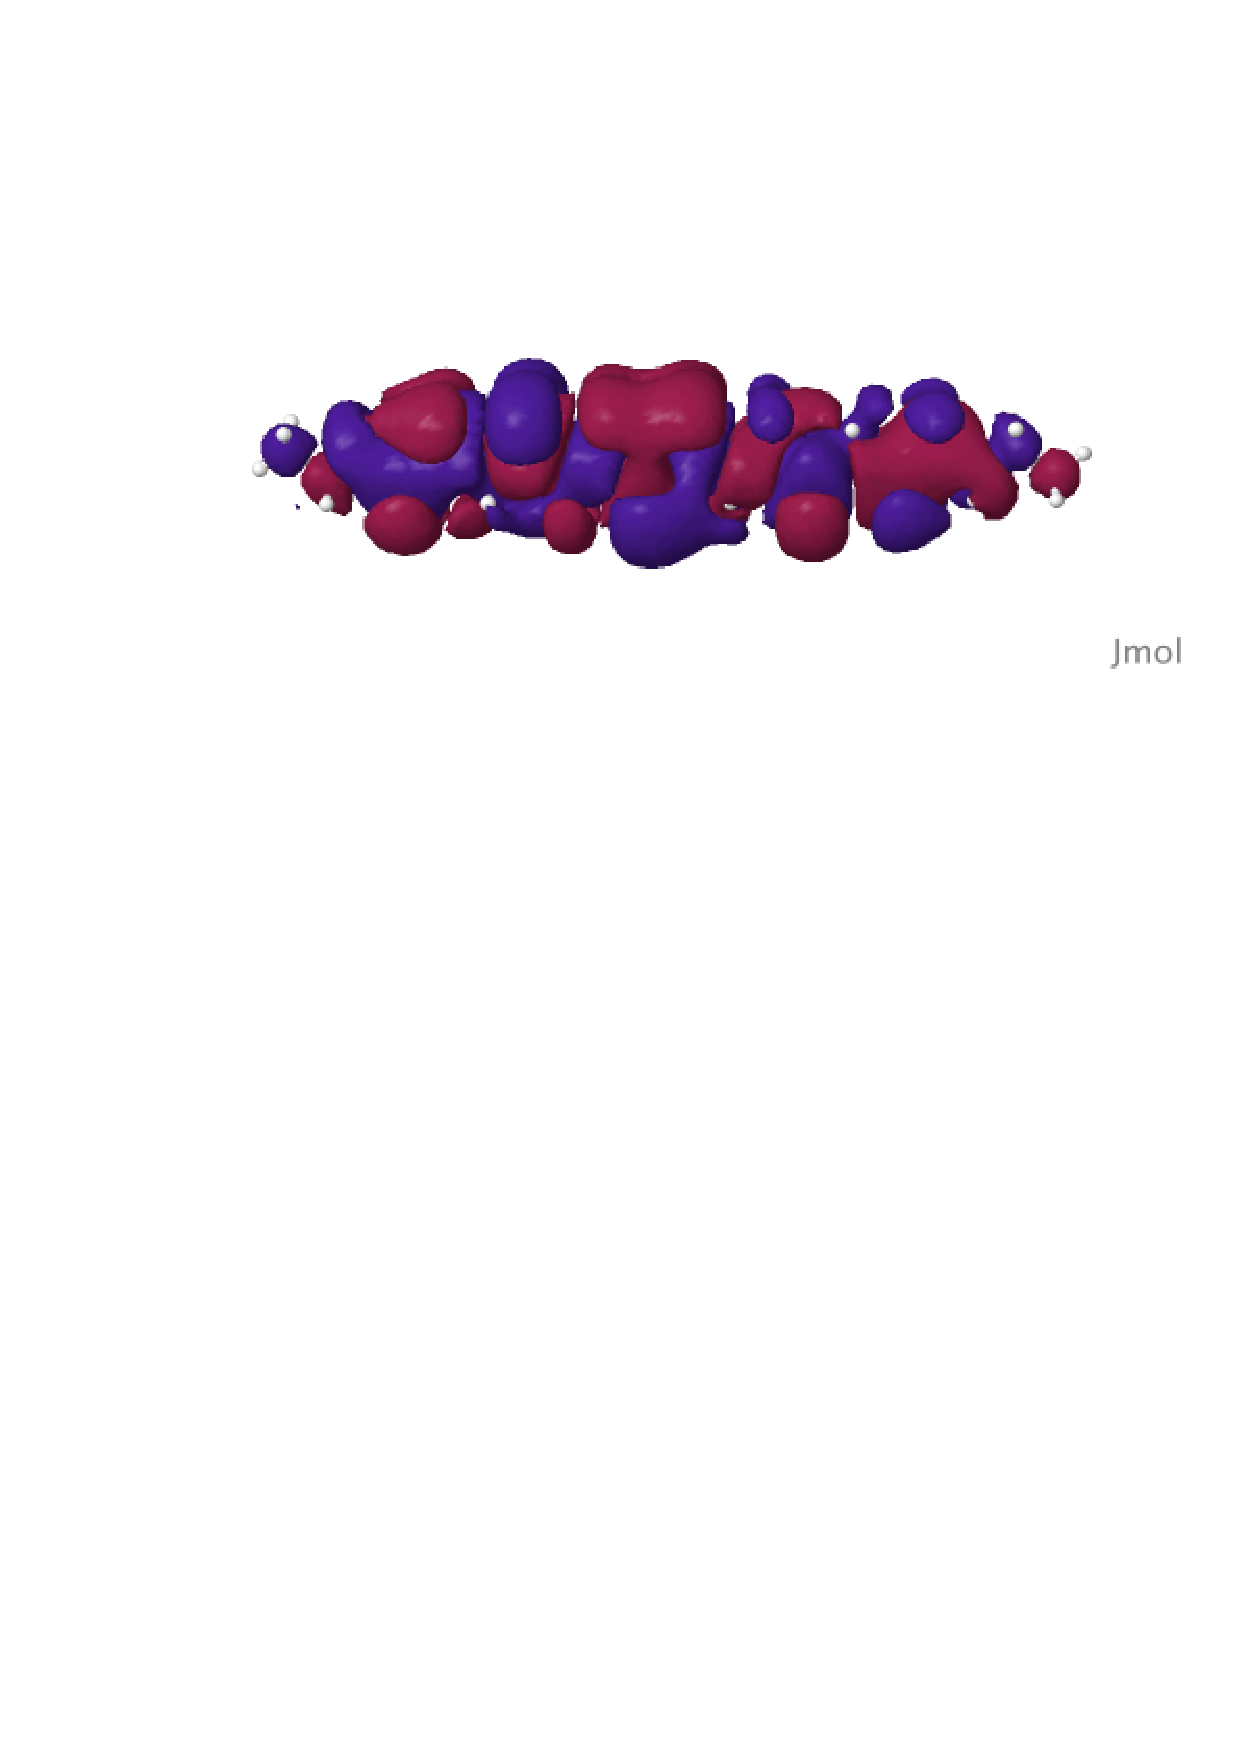
\includegraphics[scale=0.25, clip, viewport = 80 560 600 700]{figures/can_orb_1.pdf}\\
    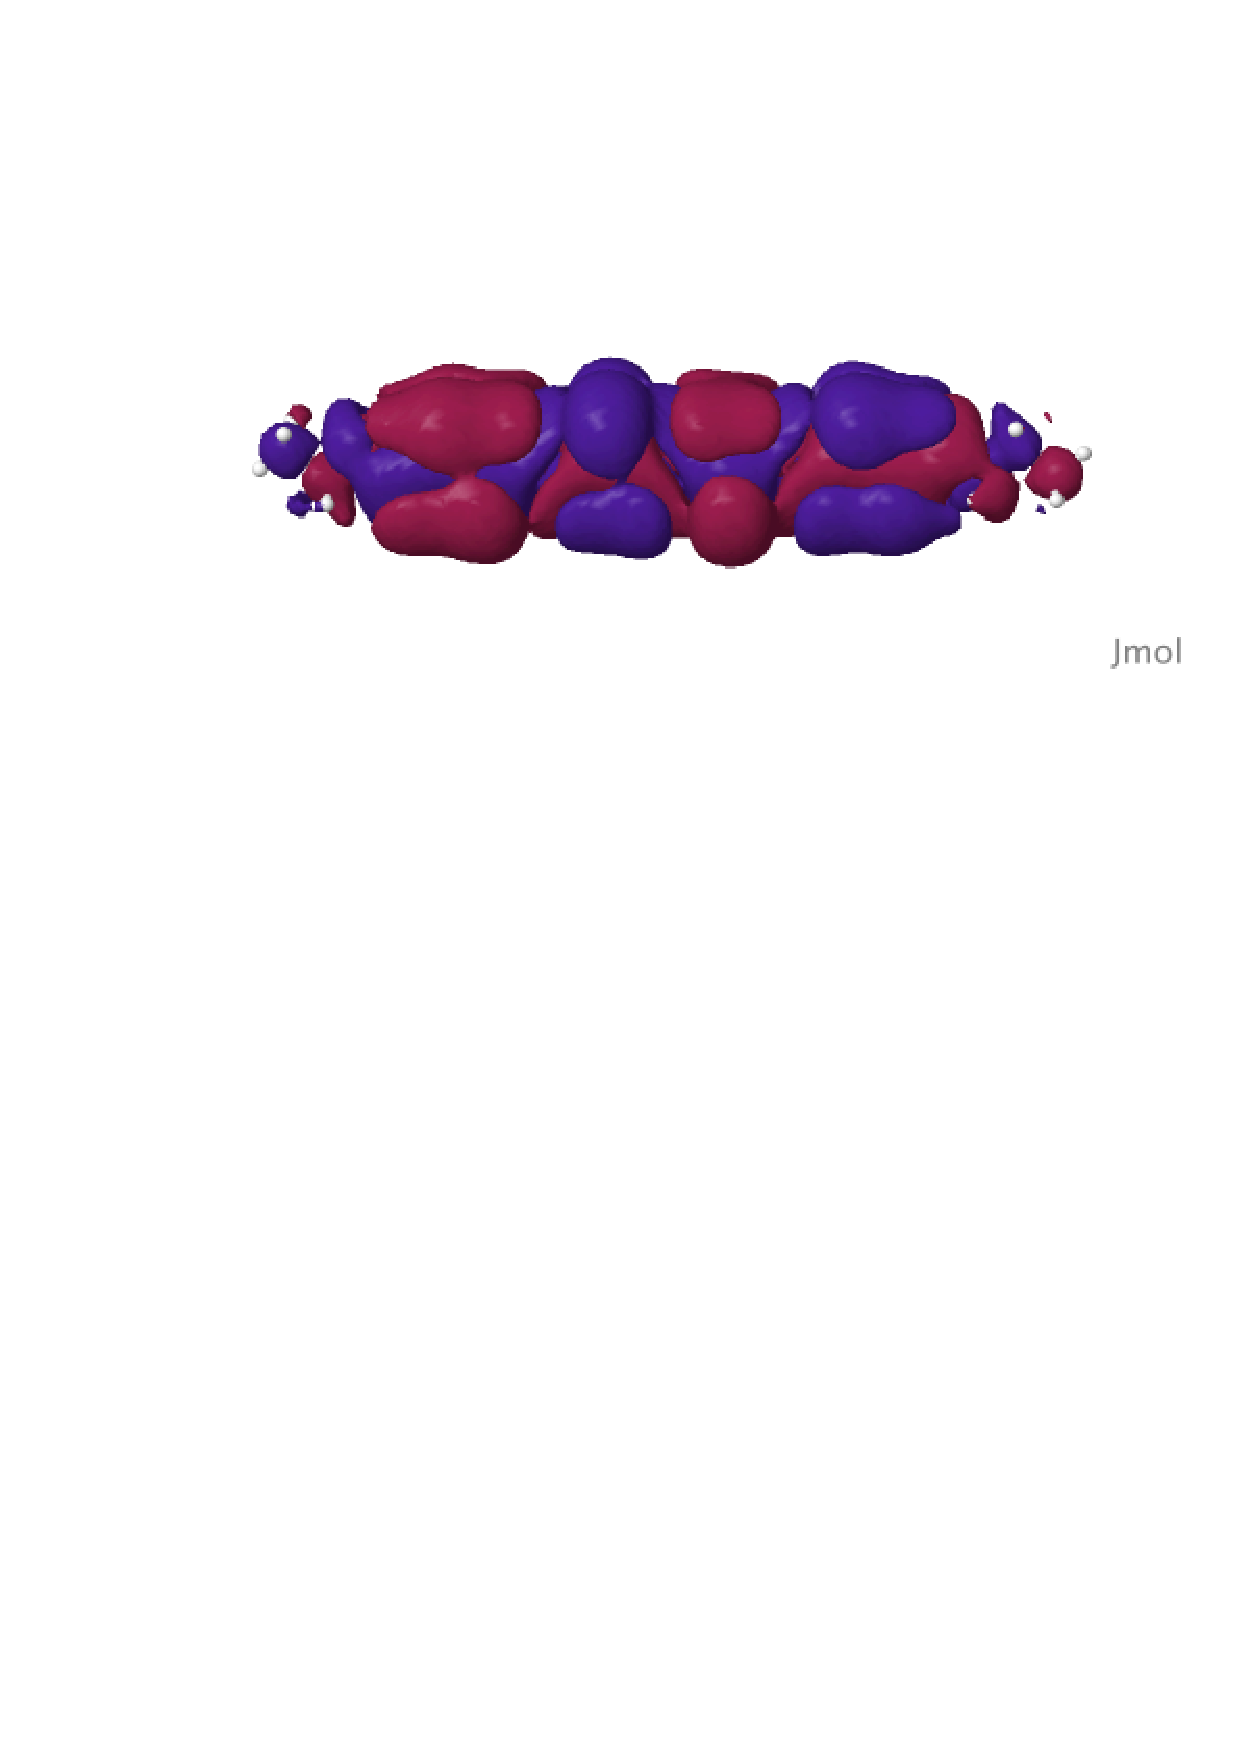
\includegraphics[scale=0.25, clip, viewport = 80 560 600 700]{figures/can_orb_2.pdf}\\

    \vspace{2mm}

    \begin{equation}
        \nonumber
        \phi_i^{n+1} =\ -2\hat{G}^n\Bigg[\hat{V}^n\phi_i^n
        - (\epsilon^n_i - \lambda^n_i)\phi_i^n\Bigg]
    \end{equation}
    \end{column}

    \begin{column}[b]{0.48\linewidth}
\only<2>{
    \centering
    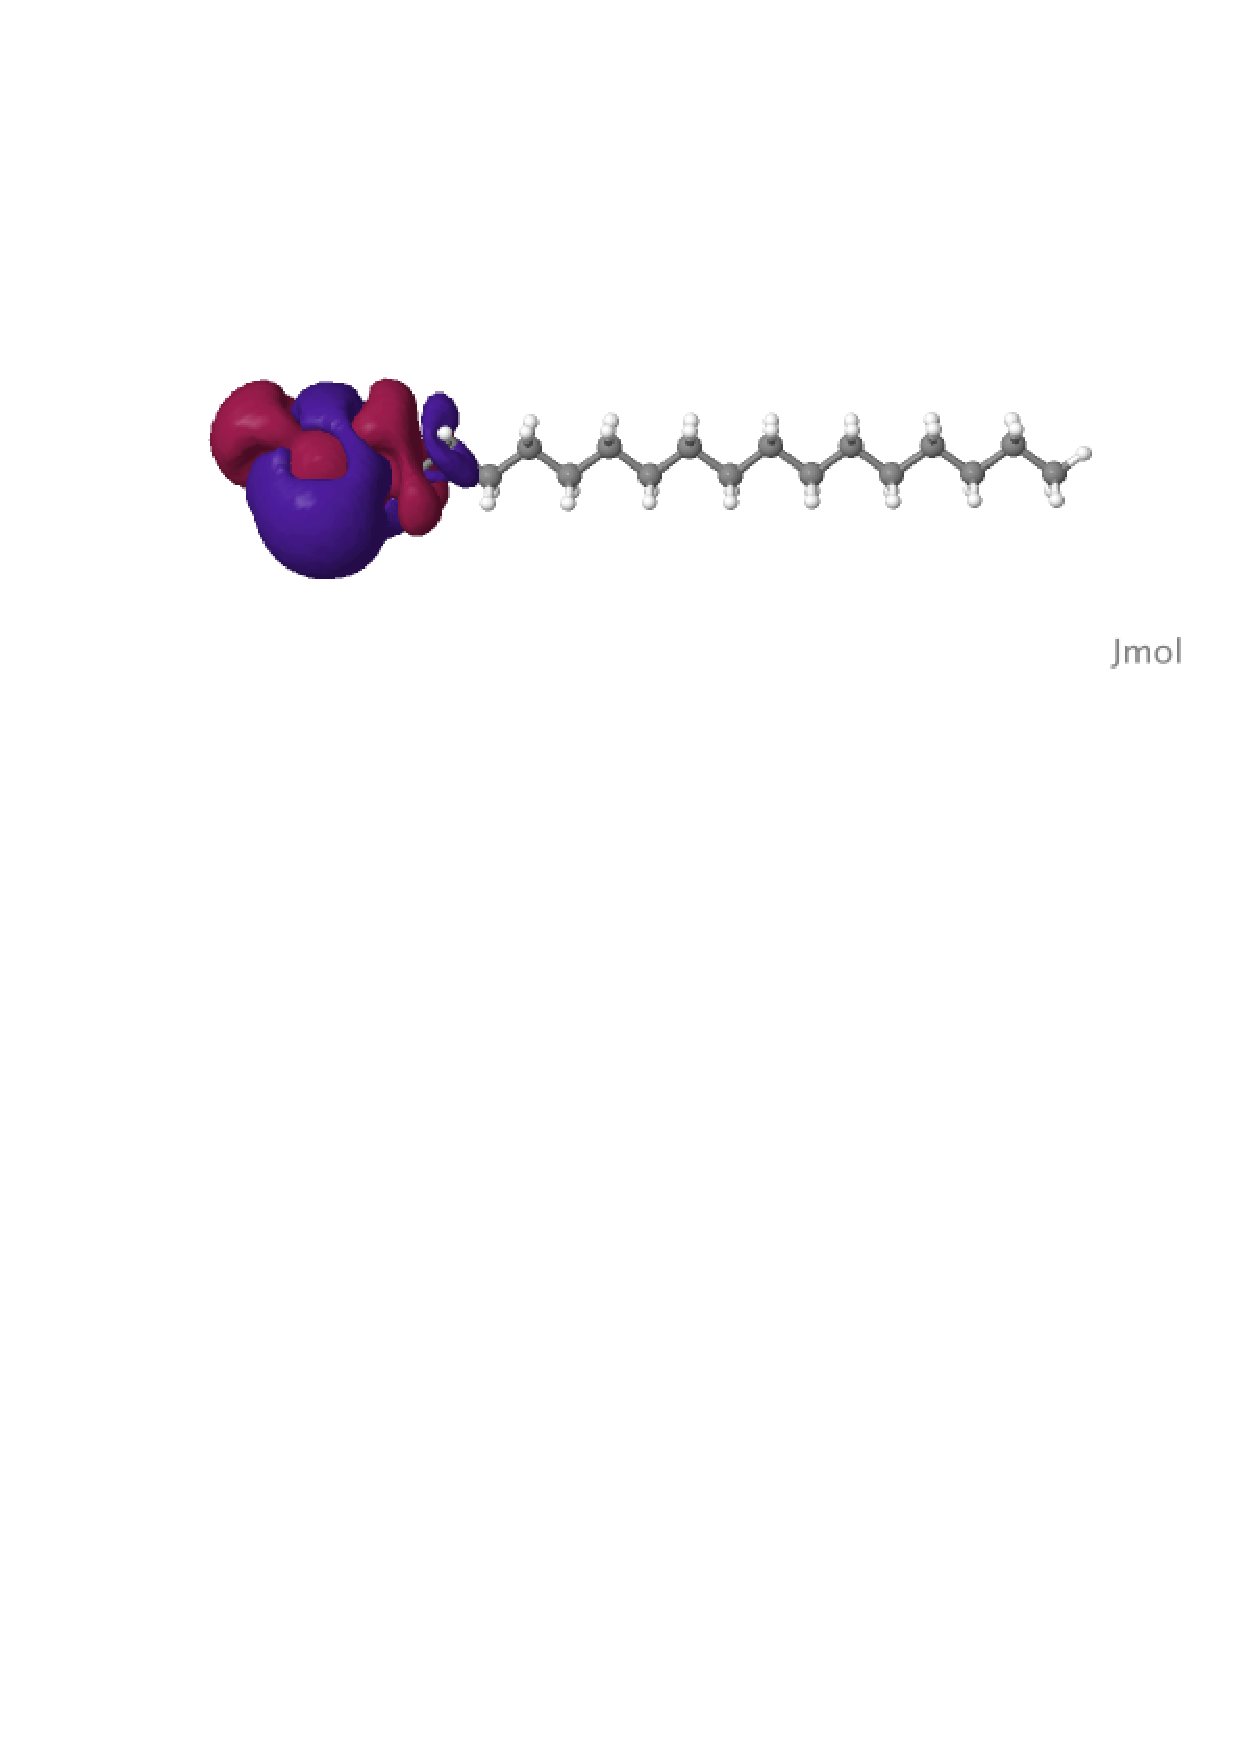
\includegraphics[scale=0.25, clip, viewport = 80 560 600 700]{figures/loc_orb_1.pdf}\\
    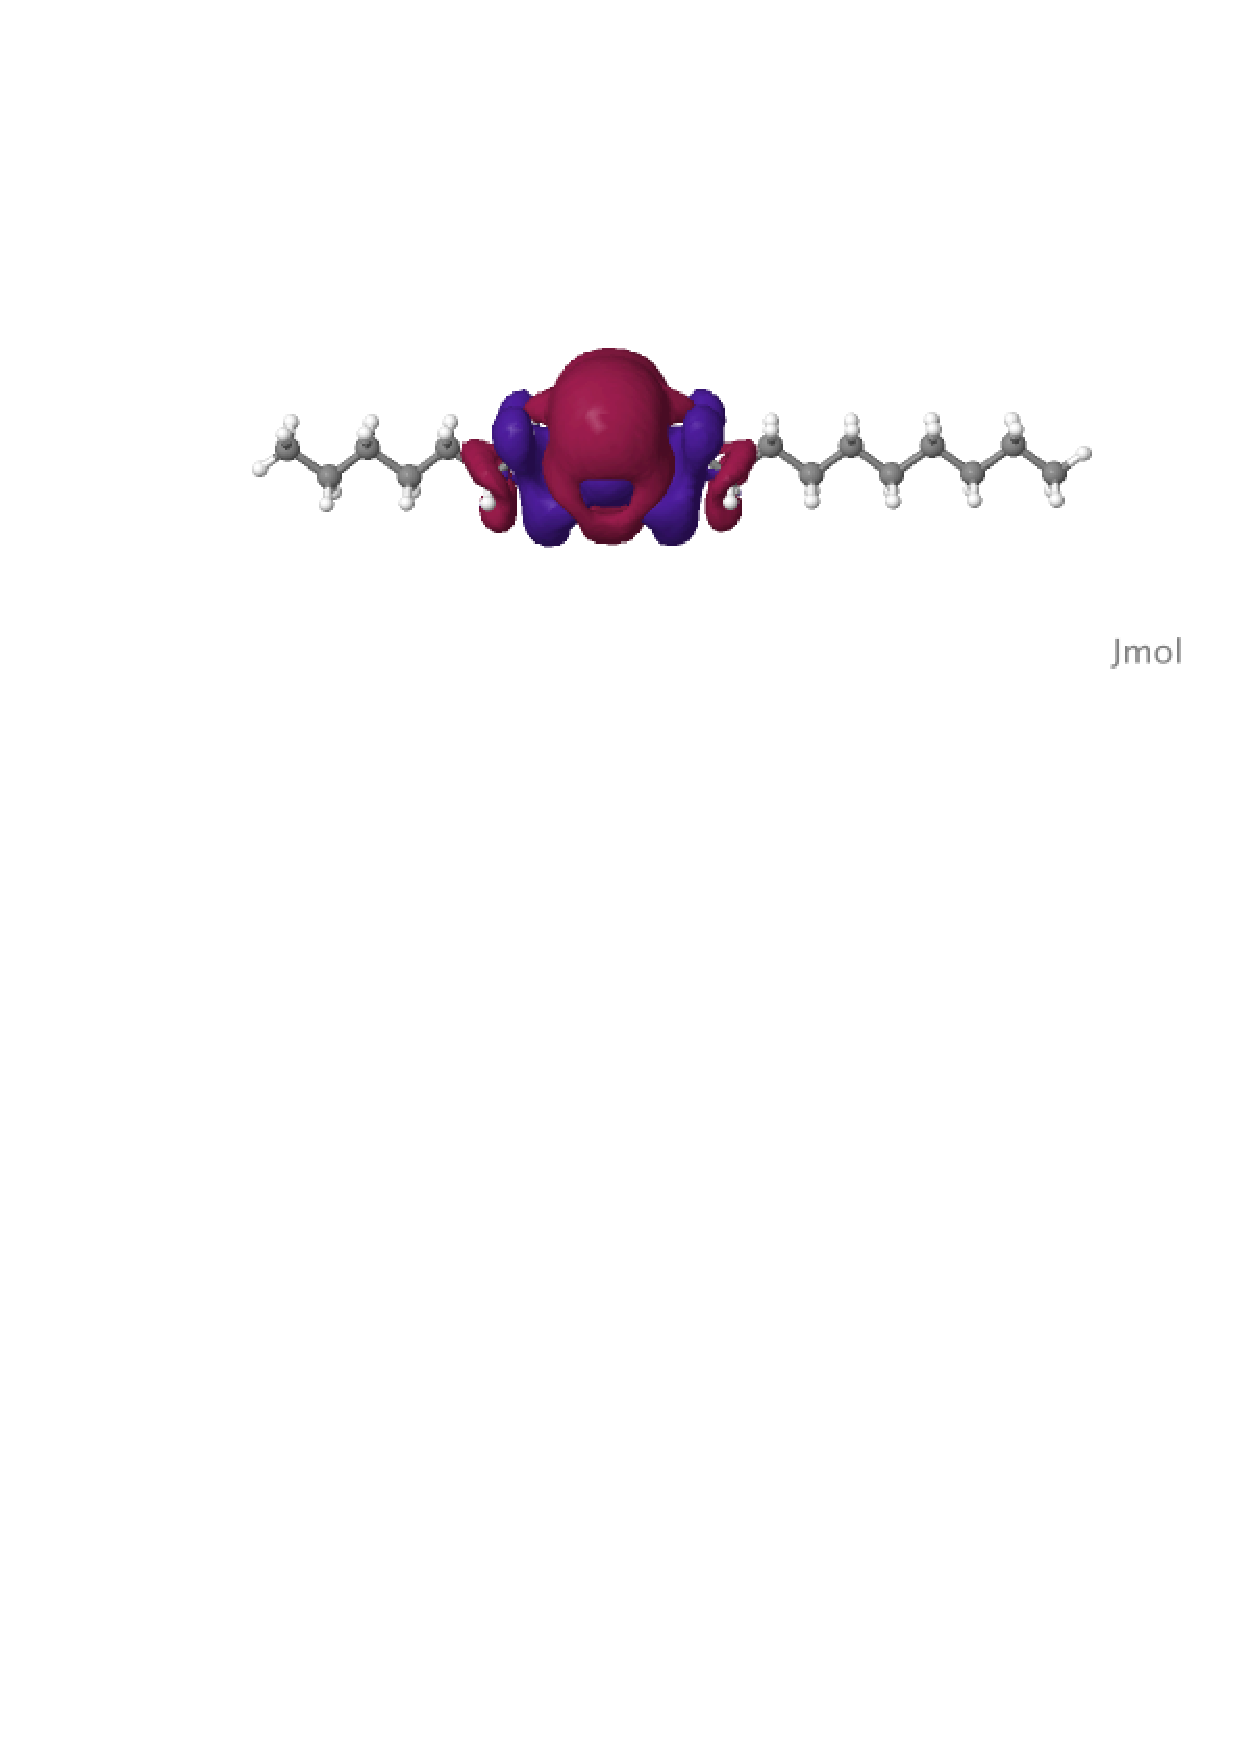
\includegraphics[scale=0.25, clip, viewport = 80 560 600 700]{figures/loc_orb_2.pdf}\\
    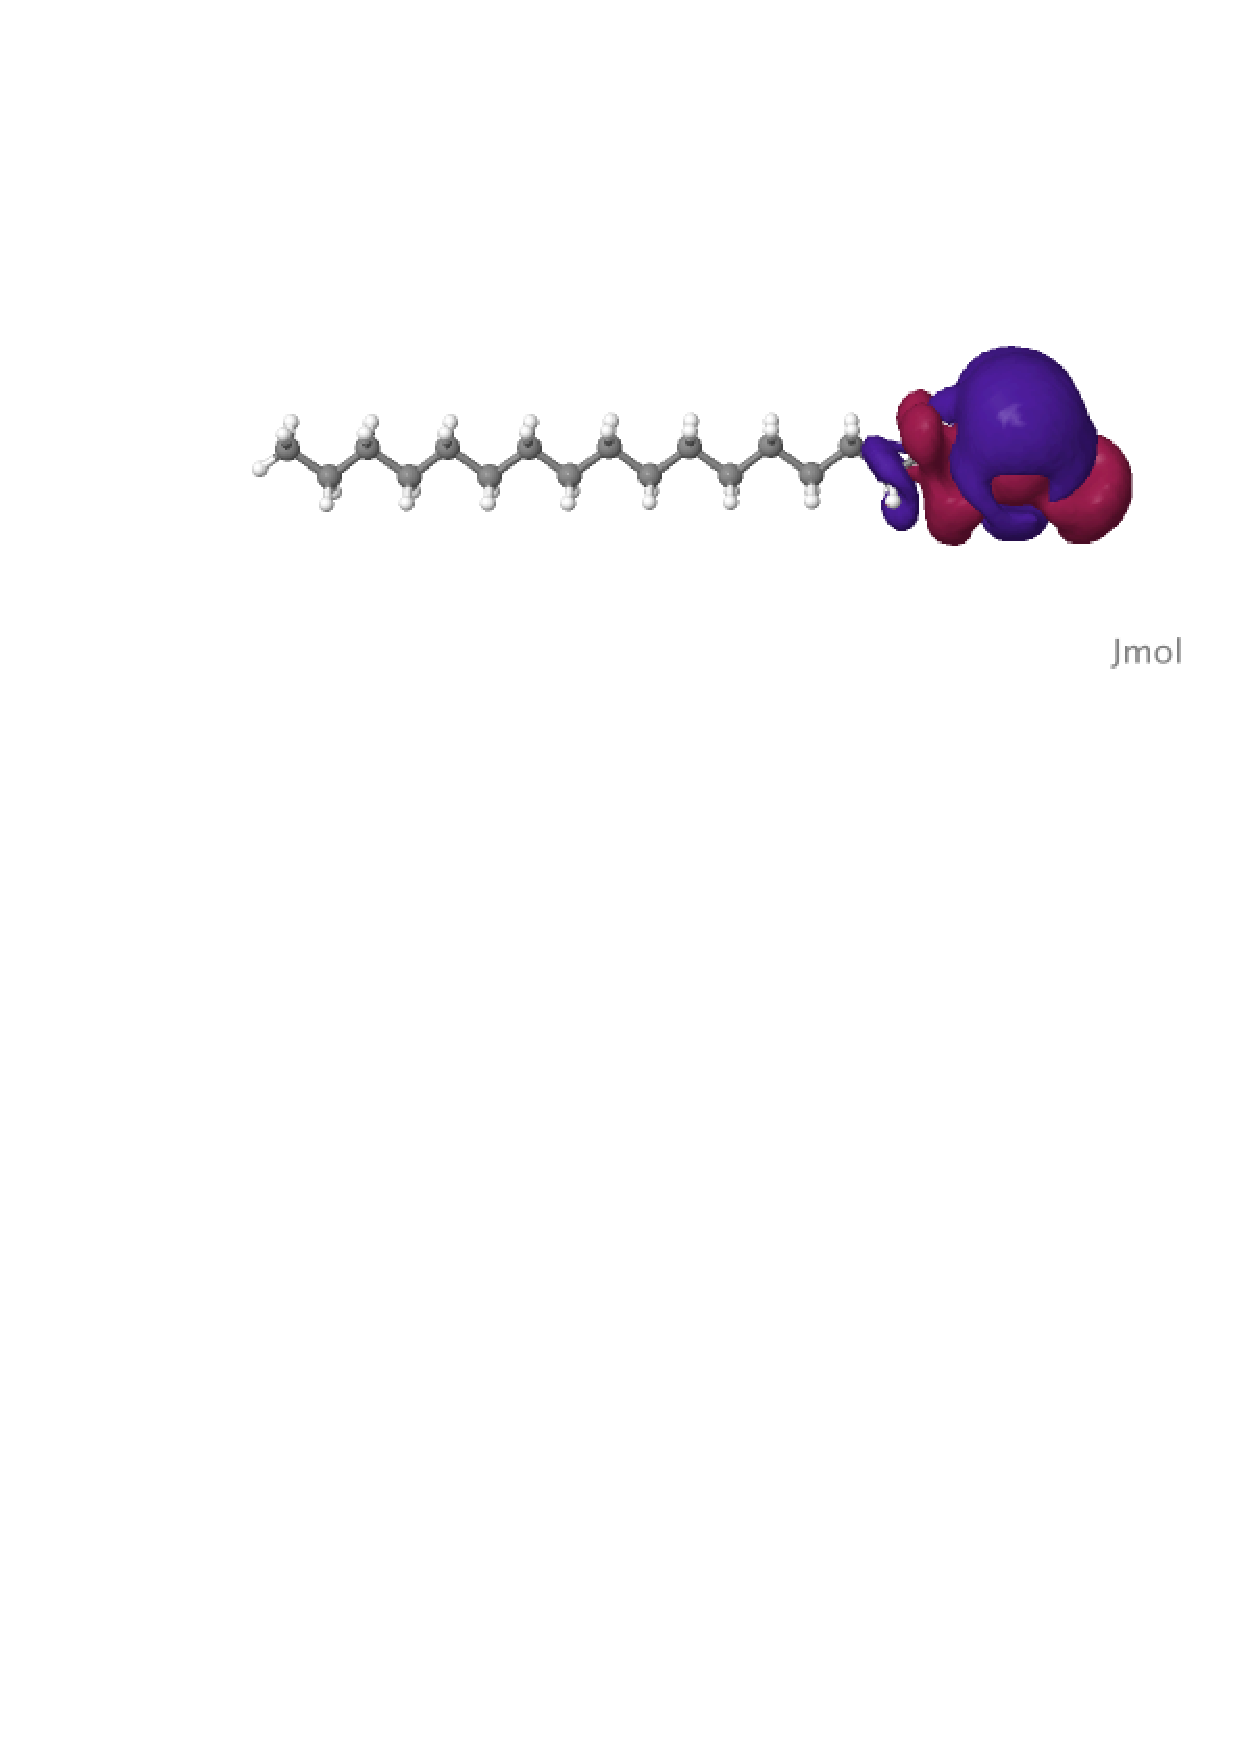
\includegraphics[scale=0.25, clip, viewport = 80 560 600 700]{figures/loc_orb_3.pdf}\\

    \vspace{2mm}

    \begin{equation}
        \nonumber
        \phi_i^{n+1} =\ -2\hat{G}^n\Bigg[\hat{V}^n\phi_i^n
        - \sum_j(F^n_{ij} - \Lambda^n_{ij})\phi_j^n\Bigg]
    \end{equation}
}
    \end{column}
    \end{columns}

    \vspace{6mm}

    \centering
    \tiny
    S.F. Boys,
    {\it Rev. Mod. Phys.}, 
    \textbf{32:296}
    (1960)\\
    J.M. Foster, S.F. Boys,
    {\it Rev. Mod. Phys.}, 
    \textbf{32:300}
    (1960)
\end{frame}

\begin{frame}
    \frametitle{Orthonormalization}
    \centering
    \textbf{The non-canonical Kohn-Sham equations}
    \begin{equation}
        \nonumber
        \tilde{\phi}_i^{n+1} = -2\hat{G}^n \bigg[\hat{V}^n\phi_i^n -
        \sum_j\big(F_{ij} - \Lambda_{ij}\big)\phi_j\bigg]
    \end{equation}
    
    \vspace{10mm}

    \textbf{Overlap matrix}
    \begin{equation}
        \nonumber
        \tilde{S}_{ij} = \langle\tilde{\phi}_i|\tilde{\phi}_j\rangle
    \end{equation}

    \vspace{10mm}

    \begin{columns}
    \begin{column}[b]{0.3\linewidth}
    \centering
    \textbf{Diagonalize}
    \begin{equation}
	\nonumber
        U = C\tilde{S}^{-1/2}
    \end{equation}
    \end{column}

    \begin{column}[b]{0.4\linewidth}
    \centering
    \textbf{Localize}
    \begin{equation}
	\nonumber
        U = L\tilde{S}^{-1/2}
    \end{equation}
    \end{column}

    \begin{column}[b]{0.3\linewidth}
    \centering
    \textbf{Orthonormalize}
    \begin{equation}
	\nonumber
        U = \tilde{S}^{-1/2}
    \end{equation}
    \end{column}
    \end{columns}

    \vspace{10mm}

    \centering
    \textbf{Orbital rotation}
    \begin{equation}
	\nonumber
	\phi_i = \sum_j U_{ij} \tilde{\phi}_j \qquad \qquad F = U\tilde{F}U^{-1}
    \end{equation}
\end{frame}

\begin{frame}
    \frametitle{Many-electron systems}
    SCF algorithm I
\end{frame}

\begin{frame}
    \frametitle{Many-electron systems}
    \centering
    \textbf{Overall accuracy kept at} $\epsilon = 10^{-6}$
    \begin{center}
	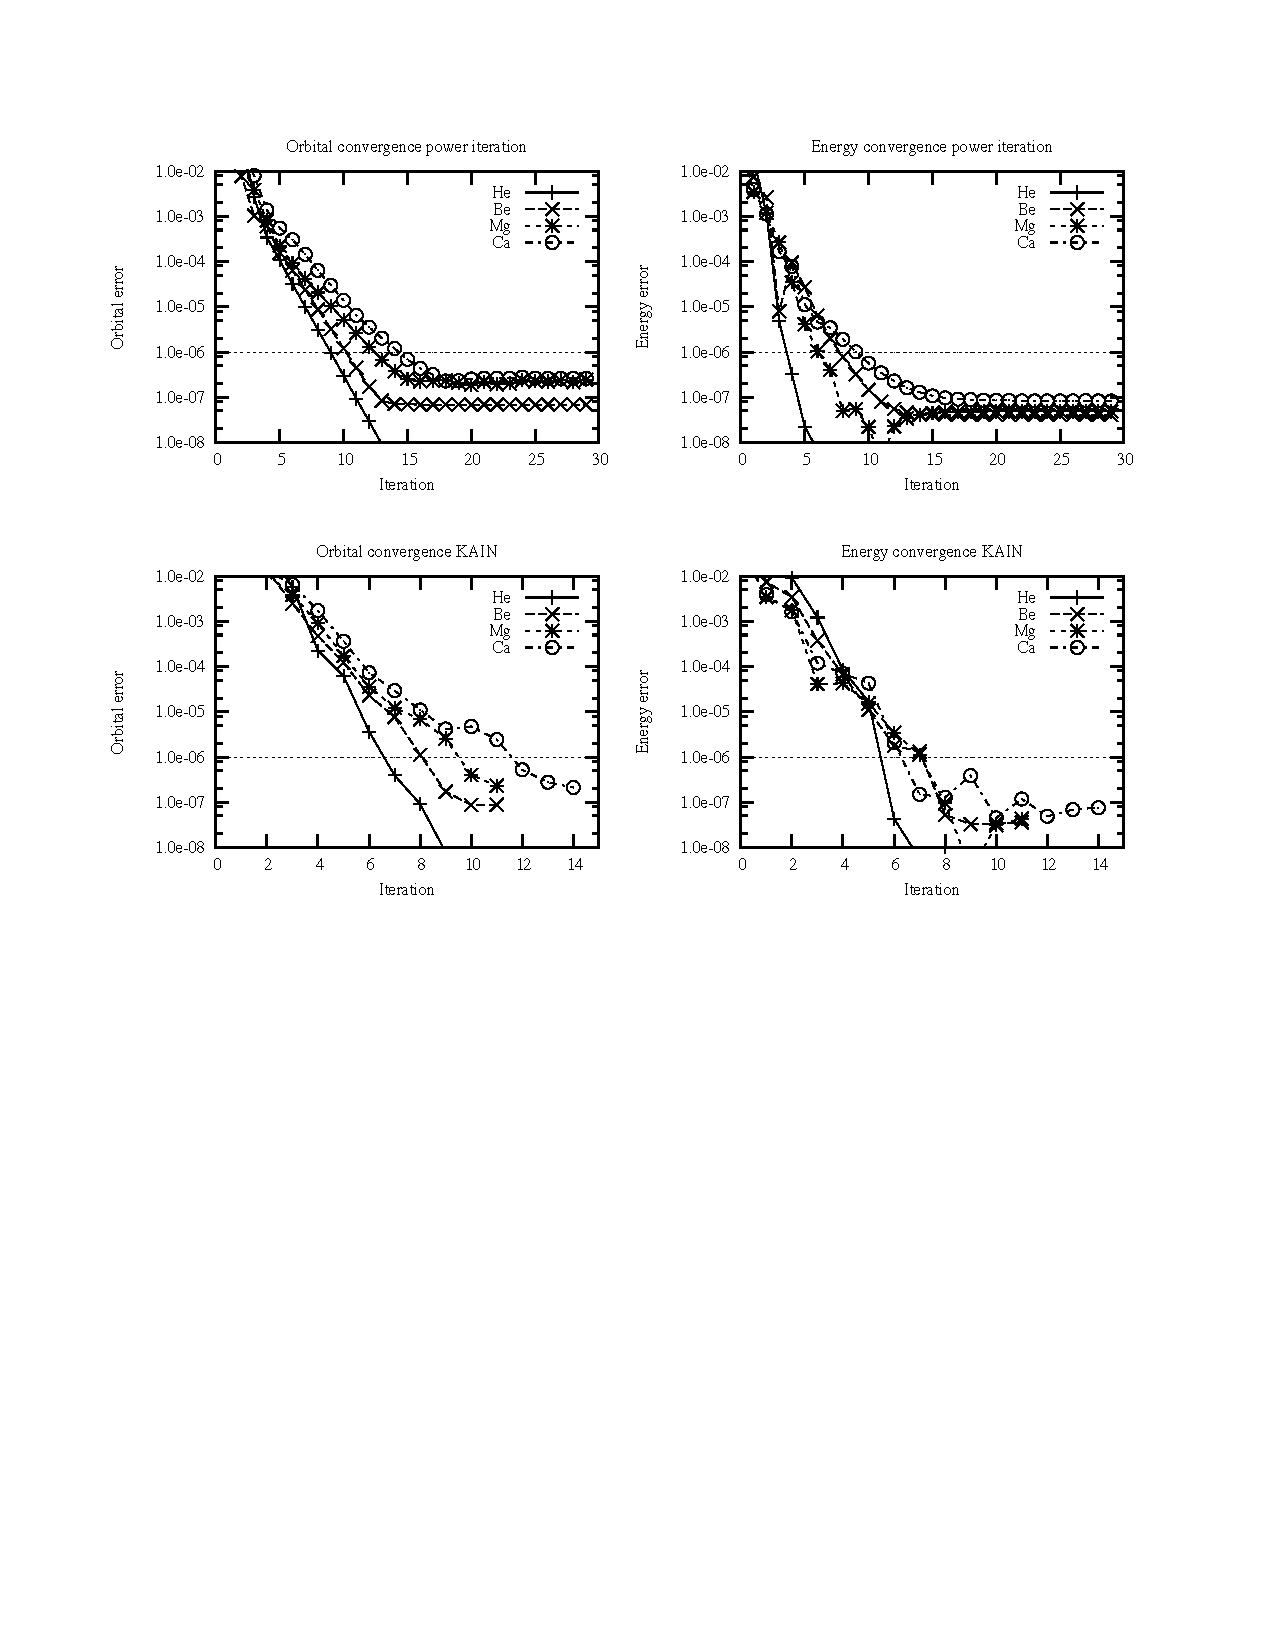
\includegraphics[scale=0.8, clip, viewport = 50 550 300 740]{figures/accuracy.pdf}
    \end{center}
\end{frame}

\begin{frame}
    \frametitle{Many-electron systems}
    Calculation of Fock matrix
\end{frame}

\begin{frame}
    \frametitle{Many-electron systems}
    SCF algorithm II
\end{frame}

\begin{frame}
    \frametitle{Many-electron systems}
    Results
\end{frame}

\begin{frame}
    \frametitle{Many-electron systems}
    \begin{columns}
    \begin{column}[b]{0.1\textwidth}
    \ \\
    \end{column}
    \begin{column}[b]{0.4\textwidth}
    \centering
    Density
    \begin{equation}
	\nonumber
	\rho^n(\boldsymbol{r}) = \sum_i |\phi_i^n(\boldsymbol{r})|^2
    \end{equation}
    \end{column}
    \begin{column}[b]{0.4\textwidth}
    \centering
    Potentials
    \begin{equation}   
	\nonumber
	\rho^n(\boldsymbol{r}) \rightarrow v_{eff}^n(\boldsymbol{r})
    \end{equation}
    \end{column}
    \begin{column}[b]{0.1\textwidth}
    \ \\
    \end{column}
    \end{columns}
    \ \\
    \ \\
    \begin{columns}
    \begin{column}[b]{0.1\textwidth}
    \ \\
    \end{column}
    \begin{column}[b]{0.4\textwidth}
    \centering
    Power iteration
    \begin{equation}
	\nonumber
	\tilde{\phi}_i^n = -2\hat{H}\left[v_{eff}^n\phi_i^n\right]
    \end{equation}
    \end{column}
    \begin{column}[b]{0.4\textwidth}
    \centering
    Calculate updates
    \begin{equation}
	\nonumber
	\Delta\phi^n = \tilde{\phi}^n - \phi^n
    \end{equation}
    \end{column}
    \begin{column}[b]{0.1\textwidth}
    \ \\
    \end{column}
    \end{columns}
    \ \\
    \ \\
    \pause
    \only<1,2>{
    \centering
    \ \\
    \textbf{Complicating issues}
    \ \\
    \begin{columns}
    \begin{column}[b]{0.25\textwidth}
    \ \\
    \end{column}
    \begin{column}[b]{0.75\textwidth}
    \begin{itemize}
	\item	Straightforward iteration will bring all\\ 
		orbitals to the lowest energy eigenfunction
	\item	Orthonormality must be imposed
	\item	Achieved by diagonalizing the Fock matrix 
    \end{itemize}
    \end{column}
    \end{columns}
    \begin{equation}
        \nonumber
        F_{ij} = \left<\phi_i|\hat{T} + v_{eff}|\phi_j\right>
    \end{equation}
    \ \\
    \ \\
    \ \\
    \ \\
    }
    \only<3,4,5>{
    \centering
    Compute Fock matrix update
    \begin{equation}
	\nonumber
	\Delta F_{ij}^n = \left<\tilde{\phi}_i^n|v_{eff}^n |\Delta\phi_j^n\right>
		        + \left<\tilde{\phi}_i^n|\Delta v_{eff}^n|\phi_j^n\right>
    \end{equation}
    \ \\
    \ \\
    \ \\
    \pause
    \pause
    \begin{columns}
    \begin{column}[b]{0.1\textwidth}
    \ \\
    \end{column}
    \begin{column}[b]{0.4\textwidth}
    \centering
    Diagonalize matrix
    \begin{equation}
	\nonumber
	F^{n+1} = M^{-1}\tilde{F}^nM
    \end{equation}
    \end{column}
    \begin{column}[b]{0.4\textwidth}
    \centering
    Rotate orbitals
    \begin{equation}
	\nonumber
	\phi_i^{n+1} = \sum_jM^{-1}_{ij}\tilde{\phi}_j^n
    \end{equation}
    \end{column}
    \begin{column}[b]{0.1\textwidth}
    \ \\
    \end{column}
    \end{columns}
    \ \\
    \ \\
    \pause
    Compute iterative subspace acceleration (KAIN or DIIS)\\
    \ \\
    Orthonormalize\\
    \ \\
    }
\end{frame}

\begin{frame}
    \frametitle{Many-electron systems}
    \begin{columns}
    \begin{column}[b]{0.20\linewidth}
	\ \\
	\ \\
    \end{column}
    \begin{column}[b]{0.30\linewidth}
    \begin{figure}
	\centering
	\includegraphics[scale=0.2, clip, viewport = 60 450 600 720]{figures/methane.pdf}\\
	\ \\
	\ \\
    \end{figure}
    \end{column}
    \begin{column}[b]{0.50\linewidth}
    \begin{figure}
	\begin{center}
	\includegraphics[scale=0.45, clip, viewport = 320 200 520 400]{figures/methaneGrid.pdf}\\
	\end{center}
    \end{figure}
    \end{column}
    \end{columns}
    \begin{center}
	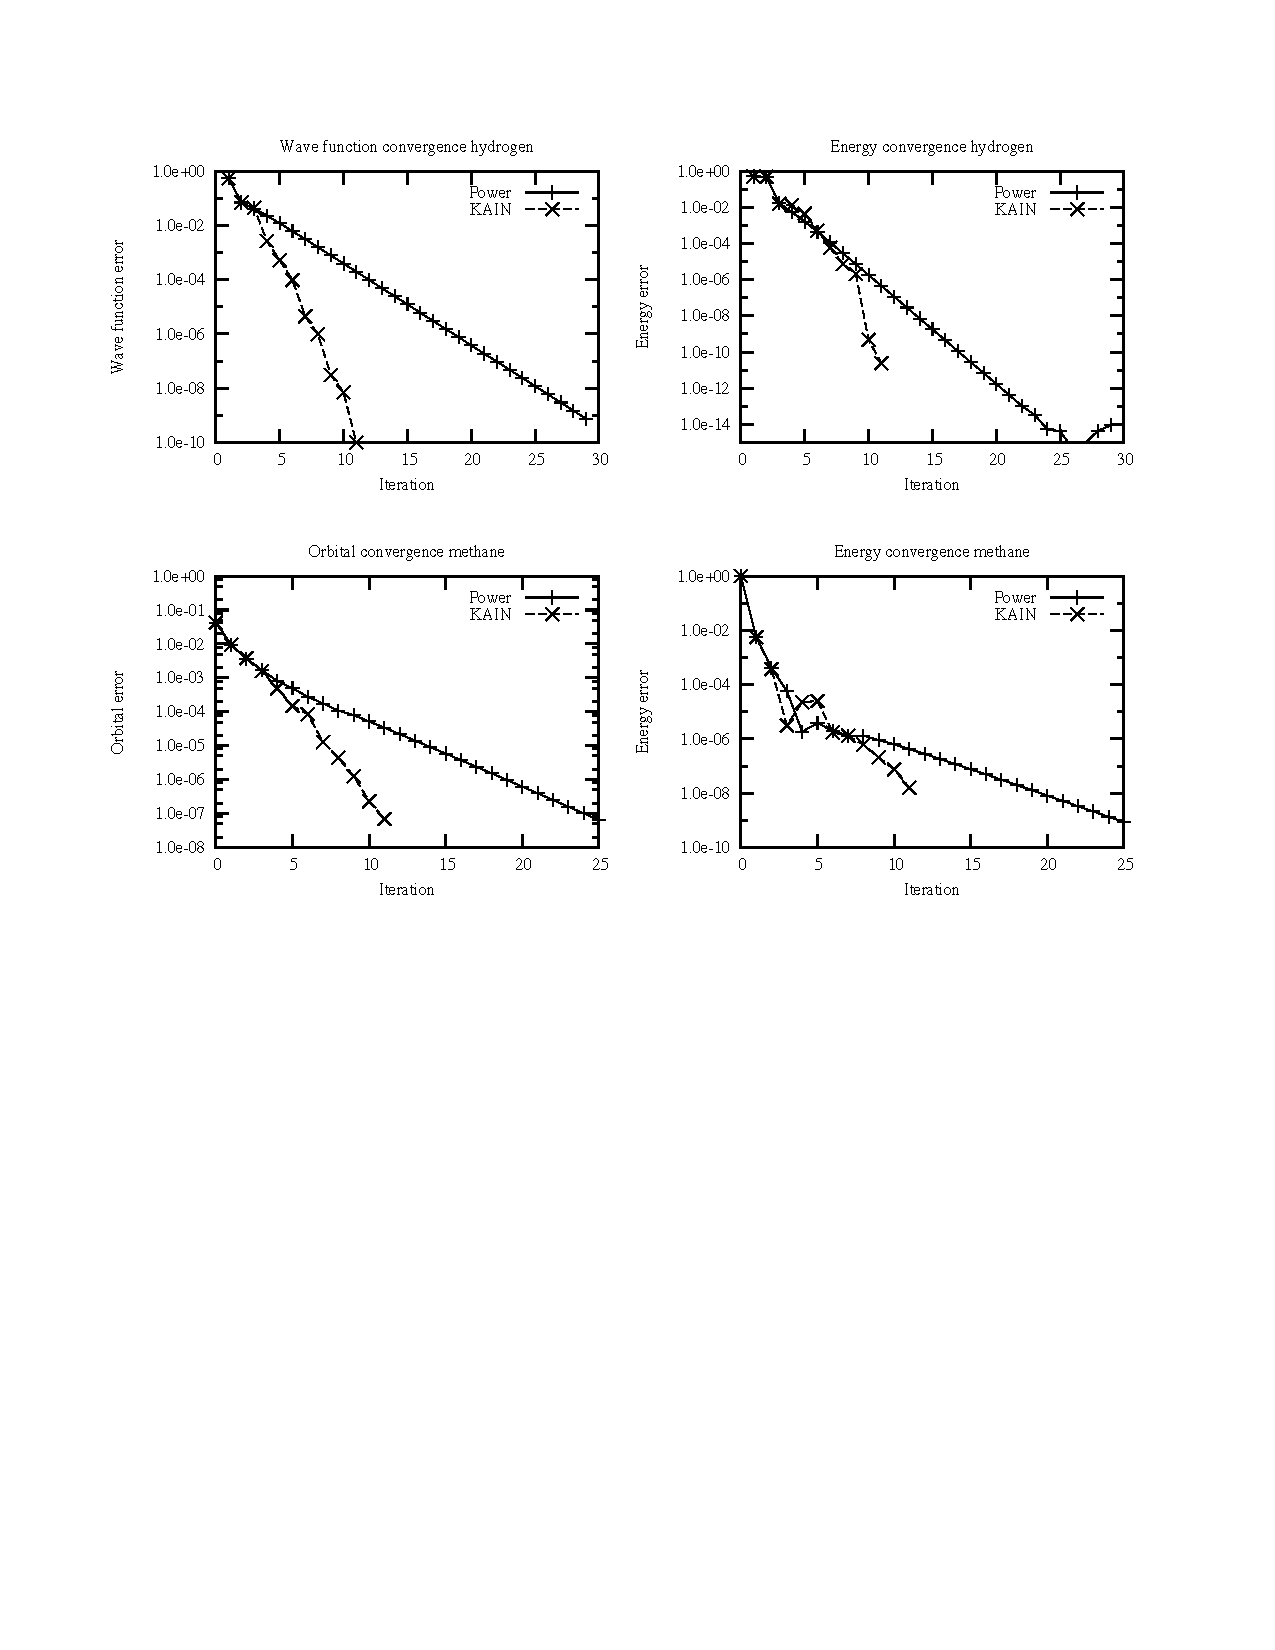
\includegraphics[scale=0.6, clip, viewport = 50 350 550 540]{figures/convergence.pdf}
    \end{center}
\end{frame}

%\begin{frame}
%    \frametitle{Accurate calculations}
%    \centering
%    LDA energies in atomic units (Hartree)
%    \begin{table}
%	\tiny
%	\centering
%        \begin{tabular}{lr@{.}lr@{.}lr@{.}lr@{.}lr@{.}lr@{.}l}
%	    \hline
%	    \hline
%	    &
%	    \multicolumn{4}{c}{Helium}&\multicolumn{4}{c}{Neon}&\multicolumn{4}{c}{Argon}\\
%	    &
%	    \multicolumn{2}{c}{HOMO}&\multicolumn{2}{c}{Total}&
%	    \multicolumn{2}{c}{HOMO}&\multicolumn{2}{c}{Total}&
%	    \multicolumn{2}{c}{HOMO}&\multicolumn{2}{c}{Total}\\
%	    \hline
%	    &\multicolumn{4}{c}{}&\multicolumn{4}{c}{}&\multicolumn{4}{c}{}\\
%	    MRChem $\epsilon=10^{-3}$&	-0&570467&-2&8348568&-0&496833&-128&262186&-0&387692&-525&966790\\
%	    MRChem $\epsilon=10^{-5}$&	-0&570424&-2&8348352&-0&498035&-128&233472&-0&382348&-525&946109\\
%	    MRChem $\epsilon=10^{-7}$&	-0&570425&-2&8348836&-0&498034&-128&233481&-0&382330&-525&946196\\
%	    &\multicolumn{4}{c}{}&\multicolumn{4}{c}{}&\multicolumn{4}{c}{}\\
%	    NIST&			-0&570425&-2&8348836&-0&498034&-128&233481&-0&382330&-525&946195\\
%	    &\multicolumn{4}{c}{}&\multicolumn{4}{c}{}&\multicolumn{4}{c}{}\\
%	    aug-cc-pV6Z&		-0&570424&-2&8348289&-0&498027&-128&233402&-0&382323&-525&944181\\
%	    aug-cc-pV5Z&		-0&570417&-2&8347859&-0&498059&-128&232889&-0&382388&-525&942021\\
%	    aug-cc-pVQZ&		-0&570406&-2&8346891&-0&498302&-128&229212&-0&382463&-525&938021\\
%	    aug-cc-pVTZ&		-0&570260&-2&8343489&-0&498859&-128&218459&-0&382838&-525&933682\\
%	    aug-cc-pVDZ&		-0&569386&-2&8291516&-0&498201&-128&176831&-0&382143&-525&915702\\
%	    &\multicolumn{4}{c}{}&\multicolumn{4}{c}{}&\multicolumn{4}{c}{}\\
%	    \hline
%	    \hline
%	\end{tabular}
%    \end{table}
%    \it{NIST: National Institute of Standards and Technology (Basis set limit)}\\
%\ \\
%\ \\
%\ \\
%\begin{itemize}
%    \item We are able to attain \textbf{considerably higher} accuracy than high-quality Gaussian basis sets
%    \item Energies are not variational, but \textbf{basis set limit} within the requested precision
%    \item Calculations are still more expensive than conventional methods
%\end{itemize}
%\end{frame}

%\begin{frame}
%    \frametitle{Accurate calculations}
%    \centering
%    Replacing the exchange-correlation potential $v_{xc}$ with the exact exchange operator
%    \begin{equation}
%	\nonumber
%	\hat{K}\phi_i(\boldsymbol{r}) = \sum_j \phi_j(\boldsymbol{r}) \int P(\boldsymbol{r}-\boldsymbol{r}')
%	    \left[\phi_i(\boldsymbol{r}')\phi_j(\boldsymbol{r}')\right] d\boldsymbol{r}'
%    \end{equation}
%    gives the Hartree-Fock equations, which can be solved by the same iterative methods
%    \ \\
%    \ \\
%\begin{table}
%\tiny
%\begin{tabular}{cllll}
%\hline   
%\hline
%\multicolumn{5}{c}{Total Hartree-Fock energies in atomic units (Hartree)}\\
%&\multicolumn{1}{c}{H$_2$O}
%&\multicolumn{1}{c}{H$_2$O$_2$}
%&\multicolumn{1}{c}{CO}
%&\multicolumn{1}{c}{CO$_2$}\\
%\hline 
%            		    &               &               &               &               \\
%MRChem $\epsilon=10^{-5}$   & -76.067611455 & -150.85253297 & -112.79087294 & -187.72538886 \\
%MRChem $\epsilon=10^{-6}$   & -76.067556696 & -150.85249254 & -112.79069389 & -187.72541991 \\
%MRChem $\epsilon=10^{-7}$   & -76.067535613 & -150.85246986 & -112.79081263 & -187.72538522 \\
%MRChem $\epsilon=10^{-8}$   & -76.067535431 & -150.85247037 & -112.79081269 & -187.72538560 \\
%            		    &               &               &               &               \\
%Est. HF limit		    & -76.0675      & -150.8525     & -112.7908     & -187.7254     \\
%            		    &               &               &               &               \\
%aug-cc-pCV5Z		    & -76.067379371 & -150.85218780 & -112.79063514 & -187.72508317 \\
%aug-cc-pCVQZ		    & -76.066140457 & -150.84985235 & -112.78919290 & -187.72260431 \\
%            		    &               &               &               &               \\
%\hline   
%\hline   
%\end{tabular}
%\end{table}
%\ \\
\ \\
%\ \\
%\begin{itemize}
%    \item We are able to attain \textbf{considerably higher} accuracy than high-quality Gaussian basis sets
%    \item Energies are not variational, but \textbf{basis set limit} within the requested precision
%    \item Calculations are still more expensive than conventional methods
%\end{itemize}
%\end{frame}

\end{document}
